%
%\documentclass[10pt]{IEEEtran}
%\usepackage{amsmath}
%\usepackage{cite}
%\usepackage{ifthen}
%\usepackage{seg}
%\usepackage{color}
%\usepackage{graphicx}
%\usepackage{subfloat}
%\usepackage{algorithm}
%\usepackage{algpseudocode}
%
%\DeclareRobustCommand{\dlo}[1]{}
%\DeclareRobustCommand{\wen}[1]{#1}
%\DeclareRobustCommand{\old}[1]{}
%\DeclareRobustCommand{\new}[1]{#1}
%
%\begin{document}
\DeclareRobustCommand{\old}[1]{}
\DeclareRobustCommand{\new}[1]{#1}
\DeclareRobustCommand{\dlo}[1]{}
\DeclareRobustCommand{\wen}[1]{#1}


\published{IEEE Transactions on Geoscience and Remote Sensing, xxx, xxx, (2021)}

\title{Statistics-guided residual dictionary learning for 
footprint noise removal}
\author{Wei Chen\footnotemark[1]\footnotemark[2], Omar M. Saad\footnotemark[1], Hang Wang\footnotemark[4], and Yangkang Chen\footnotemark[1]}

\renewcommand{\thefootnote}{\fnsymbol{footnote}}

\ms{TGRS-2021} 

\address{
\footnotemark[1]
Key Laboratory of Exploration Technology for Oil and Gas Resources\\
Ministry of Education\\
Yangtze University\\
\footnotemark[2]
Hubei Cooperative Innovation Center of Unconventional Oil and Gas\\
Yangtze University \\
\footnotemark[3]
School of Earth Sciences\\
Zhejiang University\\
Hangzhou, Zhejiang Province, China, 310027\\
\footnotemark[4]
ENSN Laboratory\\
Seismology Department\\
National Research Institute of Astronomy and Geophysics (NRIAG), Egypt
}

\lefthead{Chen et al., 2021}
\righthead{Footprint noise removal}
%\thanks{This work was supported in part by the National Natural Science Foundation of China (NSFC) under Grant 41804140, and in part by the Open Fund of Cooperative Innovation Center of Unconventional Oil and Gas (Ministry of Education and Hubei Province), Yangtze University, under Grant UOG2020-01. (Corresponding author: Wei Chen.)}}


\maketitle

\begin{abstract}
The footprint noise is a type of coherent noise that arises from the acquisition geometry. The footprint noise is commonly seen in 3D seismic volumes and greatly affects the amplitude-based processing and interpretation steps in the seismic exploration workflow. Thus, removal of the footprint noise is necessary for warranting a reliable interpretation output of seismic data processing. However, because footprint noise is usually weak and also spatially coherent, it is inevitable to cause damages to useful signals during its removal steps. Here, we propose a dictionary learning based method to effectively remove the footprint noise. We design an algorithm framework to effectively learn the dictionary atoms of the signal waveforms and separate the features of the footprint noise from the learned atoms. Considering the special features of the footprint noise in the dictionary atoms, we propose a statistics guided way to separate the dictionary atoms into footprint-affected and footprint-free atoms. Then, the footprint-affected atoms are processed via a 2D median filtering step. The combination between the untouched footprint-free atoms and filtered footprint-affected atoms result in a better dictionary of the signal waveforms and the footprint atoms. We use residual dictionary learning to encode the input data by a linear combination of signal atoms and footprint atoms. Removal of footprint atoms and their corresponding sparse coefficients leads to a successful footprint removal. We use both 3D synthetic and field data examples to demonstrate the effectiveness of the proposed method.
\end{abstract}

%\begin{keywords}
%Seismic signal processing, dictionary learning, seismic amplitude, footprint
%\end{keywords}

\section{Introduction}
Enhancing the signal-to-noise ratio of seismic data is a very common topic that will never be out-of-date in the community of exploration geophysics. Noise that exists inevitably in the seismic data can be roughly divided into two categories, i.e., incoherent and coherent noise. Both of them may cause the degradation of the final imaging of geology structures if not handled properly. Thus, many denoising algorithms based on different mathematical fundamentals have been proposed to eliminate those noise, such as the sparse transforms \cite{Yaru2014Radon,Benfeng2014POCS,mostafa2017geo,Min2019Gaussian}, rank-reduction methods \cite{Yangkang2016drr,Yangkang2019orr}, prediction based methods \cite{Spitz1991fx,Chao2018Adap,Guochang2019Multi}, dictionary-learning based methods \cite{yangkang2016double,amir2017geo,amir2017,yangkang2019sparse}, and so on. Among many kinds of coherent noise, footprint is a very special one \cite{Marfurt1998ft}. It is mainly caused by the inherent drawbacks of the acquisition geometry, such as the irregular source-receiver position, insufficient spatial sampling rate and nonuniform fold number, which further lead to the regular but unwanted amplitude variation in the seismic profile (or 3D volume). This abnormal variation that is not caused by the subsurface structures will have some negative impacts on the subsequent geological interpretation since the footprint coherency may get mixed with that of signal and thus, is mistaken for the geological structure. Therefore, removing this kind of coherent noise is of great importance.

In the past decades, many researchers have observed the footprint noise in different types of seismic data, and analyzed features and causes of it \cite{Stephen1999plot,John2001ft,Jingye2008tow}. Marfurt et al. (1998) \cite{Marfurt1998ft} defined the footprint as the noise related to the acquisition geometry. The existence of this kind of noise may cause many troubles in calculating the seismic coherency, which further leads to the inaccurate identifications of the geological bodies, such as faults and channels. This phenomenon can be commonly seen in the sparse 3D land explorations with low fold numbers. They also showed that the proper use of 3D dip filtering could be very effective for alleviating the adverse impact of the footprint on the attribute calculation. Schuster and Liu (2001) \cite{Schuster2001ft} illustrated the relation between the footprint noise and the migration operator. Utilizing the array theorem borrowed from another subject, one can calculate the footprint noise accurately and rapidly for different array types. This allows the engineer to quickly check and design a proper acquisition system. Cooper et al. (2008) \cite{Joanna2008num} tried to use a synthetic test to simulate the formation of the footprint noise. A completed data set with very dense acquisition grids is first created as the reference, and a sparse data set is also given by extracting some traces from the former one. By comparing their imaging results, it can be concluded that the processing related artifacts appear in both the completed and decimated data. However, the amplitude variation, related to the geometry feature, is only observed in the later one. Brown (2010) \cite{Brown2010obc} analyzed the footprint noise appearing in a four-component data that are acquired in the ocean-bottom-cable (OBC) survey. He found that the appearance of the footprint is closely related to the leading receivers in the towing end of the cable. Some processing procedures for mitigating this interference are also proposed, such as surface-consistent deconvolution\old{, etc}.

The aforementioned algorithms can also effectively help attenuate the footprint noise \cite{Bannagi2005svd,Milos2007wt,Oswaldo2012ft,Abdulmohsen2016cwt}. Al-Bannagi et al. (2005) \cite{Muhammad2005tsvd} proposed to use the truncated singular value decomposition to simultaneously suppress the random and footprint noise. Falconer and Marfurt (2008) \cite{Scott2008ft} proposed an attribute based method that \old{utilizes}\new{utilized} the geometric features of the footprint noise\old{ to characterize it}. The formed noise is then adaptively subtracted from the original noisy data. Based on the new noise-free data, the attribute can be calculated more accurately. Zhang et al. (2009) \cite{Rui2009bpd} developed a Basis Pursuit (BP) algorithm to suppress the footprint noise in 3D seismic data. Instead of directly using 3D version of BP, he applied the 2D BP operator in time and spatial directions separately. This method can sufficiently eliminate footprint noise while preserving the signal details. Chen et al. (2012) \cite{Xuehua2012swt} developed a denoising algorithm based on the stationary wavelet transform to suppress the footprint noise in the 3D marine seismic volume. The key of this method is to adjust the thresholding parameters according to the data features in different time slices. This can help suppress sufficient noise while keeping the details of the signals, which further contributes to the accurate calculations of the attribute map. Considering the negative impact of footprint noise caused by the under-sampled raw data, Chopra and Marfurt (2013) \cite{Satinder2013interp} used \new{a} 5D interpolation algorithm to reconstruct the missing data, which can effectively alleviate the footprint artifact and help obtain the more accurate attribute calculation. Gorszczyk et al. (2015) \cite{Gorszczyk2015curvelet} used the 2D discrete curvelet transform to deal with the noisy seismic data acquired in the hardrock environment. By adopting a novel thresholding strategy in the transform domain, this algorithm can effectively attenuate not only the random noise but also the coherent footprint noise. Compared with the F-XY prediction based method, the new method can obtain a more satisfactory denoising result with less signal leakage. Gomez et al. (2019) \cite{Gomez2019emd} developed a novel method based on the empirical mode decomposition (EMD) to simultaneously suppress the random and footprint noise. This new decomposition filter is applied along the spatial plane, i.e., the time slice, instead of the time direction. The filter length is non-stationary in every slice and adapted according to the signal distribution. By discarding the high-frequency component, the corresponding noise can be attenuated. Three field data examples, including one 2D and two 3D cases, all indicate that the proposed empirical-mode filtering (EMF) algorithm can remove the noise sufficiently with causing negligible signal damages. Compared with the other F-X or EMD based methods, it can achieve even better results. %Gomez and Velis (2020) proposed dictionary learning frame for suppressing the footprint noise. They used the coherence-constrained dictionary learning (CDL) method to train an initial dictionary, and then used the domain transform to filter each atom, which further produces the filtered atom and its corresponding residual. %\cite{Gomez2020dl} proposed a residual dictionary denoising (RDD) framework to suppress the footprint noise in the 3D seismic data. This algorithm is based on the dictionary learning frame. First, it uses the coherence-constrained dictionary learning (CDL) method to train an initial dictionary. Then, the domain transform is used to filter each atom, which further produces the filtered atom and its corresponding residual. These two parts make up the augmented dictionary used to suppress the footprint noise. The 3D synthetic and field examples all show that it can not only separate the footprint noise accurately but also preserve the signal details well. Additionally, the algorithm needs only few training data to form the effective dictionary which can be further applied in the other data sets. This can significantly reduce the computational costs. 

Sometimes, the suppression of footprint noise appears as an important step in the inversion, migration or interpretation framework \cite{Lee2005mig}. Canning and Gardner (1988) \cite{Canning1998ft} mentioned the detrimental effects of the footprint on the 3D dip moveout and prestack migration. They proposed to change the migration procedures to better mitigate the footprint interference. Gesbert (2001) \cite{Gesbert2001ft} illustrated the reason for the appearance of footprint noise and its negative impacts on the migration imaging. By dividing the big data set into small ones and changing the quadrature way, it can output an improved migration result with the good signal fidelity. Feng et al. (2018) \cite{Feng2018deblurring} proposed to use a multiparameter deblurring filter to help the multiparameter seismic inversion. Different tests show that, by adopting this filter,  the footprint noise is effectively suppressed and the signal true amplitudes are recovered well. The overall imaging quality can get a significant improvement. Qi et al. (2018) \cite{Qi2018fault} designed an effective workflow to better identify the faults in the seismic data. One of the main steps in the proposed workflow is to attenuate the footprint noise, which creates the optimized input data for the subsequent fault detection.

In this paper, we propose a new footprint removal method based on dictionary learning. We first learn the features of the useful signals and the footprint noise, respectively, based on a statistics-guided classification scheme. Then, the learned signal and noise atoms are concatenated as an augmented dictionary, and are used to separate the signal and noise via a residual dictionary learning step. We demonstrate the performance of the proposed method via both synthetic and real data examples. 

\section{Theory}
\subsection{Dictionary learning}

Let $\mathbf{d}$ be the input seismic data. First, we apply a patching method to segment the input data into a group of patches:
\begin{equation}
\label{eq:patch}
\mathbf{Y}=p(\mathbf{d}).
\end{equation}
Supposing the patch size is $l_1\times l_2$, then each column in $\mathbf{Y}$ is of size $l_1l_2\times 1$.  $p(\cdot)$ denotes the patching process.

The goal of dictionary learning is to iteratively update a dictionary and a sparse coefficient matrix so that
\begin{equation}
\label{eq:eq2}
\mathbf{Y} \approx \mathbf{D}\mathbf{M}, \quad\text{s.t.}  \quad \forall_i ||\mathbf{m}_{i}||_{0}\le Q,
\end{equation}
where $\mathbf{D}$ is the learned dictionary and $\mathbf{M}$ is the sparse coefficient matrix\old{.}\new{,} $Q$ denotes the sparsity constraint, meaning that the number of non-zero entries of each column of $\mathbf{M}$ will be equal to Q.  

To solve equation  \ref{eq:eq2}, one needs to iteratively solve the following two problems, i.e., dictionary updating and sparse coding, respectively. 
\begin{equation}
\label{eq:dic}
\hat{\mathbf{D}}^n = \arg\min_{\mathbf{D}^n} \parallel \mathbf{Y} - \mathbf{D}^n\mathbf{M}^n \parallel_F^2, 
\end{equation}
and 
\new{\begin{equation}
\label{eq:code}
\hat{\mathbf{M}}^n = \arg\min_{\mathbf{M}^n} \parallel \mathbf{Y} - \mathbf{D}^n\mathbf{M}^n \parallel_F^2, \quad\text{s.t.}  \quad \forall_i ||\mathbf{m}_{i}||_{0}\le Q,
\end{equation}}
\new{where $n$ denotes the iteration number.}

\subsection{K-SVD-based dictionary update}
The K-SVD algorithm is one of the most widely used methods to update the dictionary. 
In the K-SVD algorithm, 
\begin{equation}
\begin{split}
\mathbf{D}^{n+1}&=\arg\min||\mathbf{Y}-\mathbf{D}\mathbf{M}^{n}||^{2}_{F}\\
&=\arg\min||\mathbf{Y}-\sum_{j=1}^{L}\mathbf{d}_{j}\mathbf{m}^{T}_{j}||^{2}_{F}\\
\end{split}\quad,
\end{equation}
where $\mathbf{d}_{j}$ and $\mathbf{m}^T_{j}$ are the $j$th column of dictionary matrix $\mathbf{D}$ and $j$th row of the sparse coefficient $\mathbf{M}$. 

One should fix the sparse coefficient $\mathbf{M}$ and update the dictionary $\mathbf{D}$ column by column, which can be expressed as follows:
\begin{equation}
\begin{split}
	\mathbf{D}		&=\arg\min||\mathbf{Y}-\sum_{j\neq k}^{L}\mathbf{d}_{j}\mathbf{m}^{T}_{j}-\mathbf{d}_{k}\mathbf{m}^{T}_{k}||^{2}_{F}\\
	&=\arg\min||\mathbf{R}_{k}-\mathbf{d}_{k}\mathbf{m}^{T}_{k}||^{2}_F\\
\end{split}
\quad ,
\end{equation}
where $\mathbf{R}_{k}$ denotes the residual between the input data $\mathbf{Y}$ and sparsely represented matrix excluding the $k$th column. Thus, the problem becomes to solve the rank-1 approximation of $\mathbf{R}_{k}$, which can be achieved by singular value decomposition (SVD). However, directly using SVD will destruct the sparse structure of the coefficient vector $\mathbf{m}^T_{k}$. To avoid that, one needs to apply a sub-sample operator to discard the columns in $\mathbf{R}_{k}$ where the corresponding entries in $\mathbf{m}_{k}$ are zero. The new error matrix and new coefficient vector thus become $\mathbf{R}^{new}_{k}$ and  $\mathbf{m}_{k}^{^Tnew}$, respectively. Then, the SVD is directly used for the rank-1 approximation. 
\begin{equation}
\text{J}=||\mathbf{R}_{k}-\mathbf{d}_{k}\mathbf{m}^T_k||_F^{2}=||\mathbf{R}_{k}^{new}-\mathbf{d}_{k}\mathbf{m}^{Tnew}_k||^{2}.
\end{equation}
After $\mathbf{D}$ is updated, the coefficient matrix is then updated via the orthonormal matching pursuit (OMP) method. 

\begin{figure}[htb!]
\centering
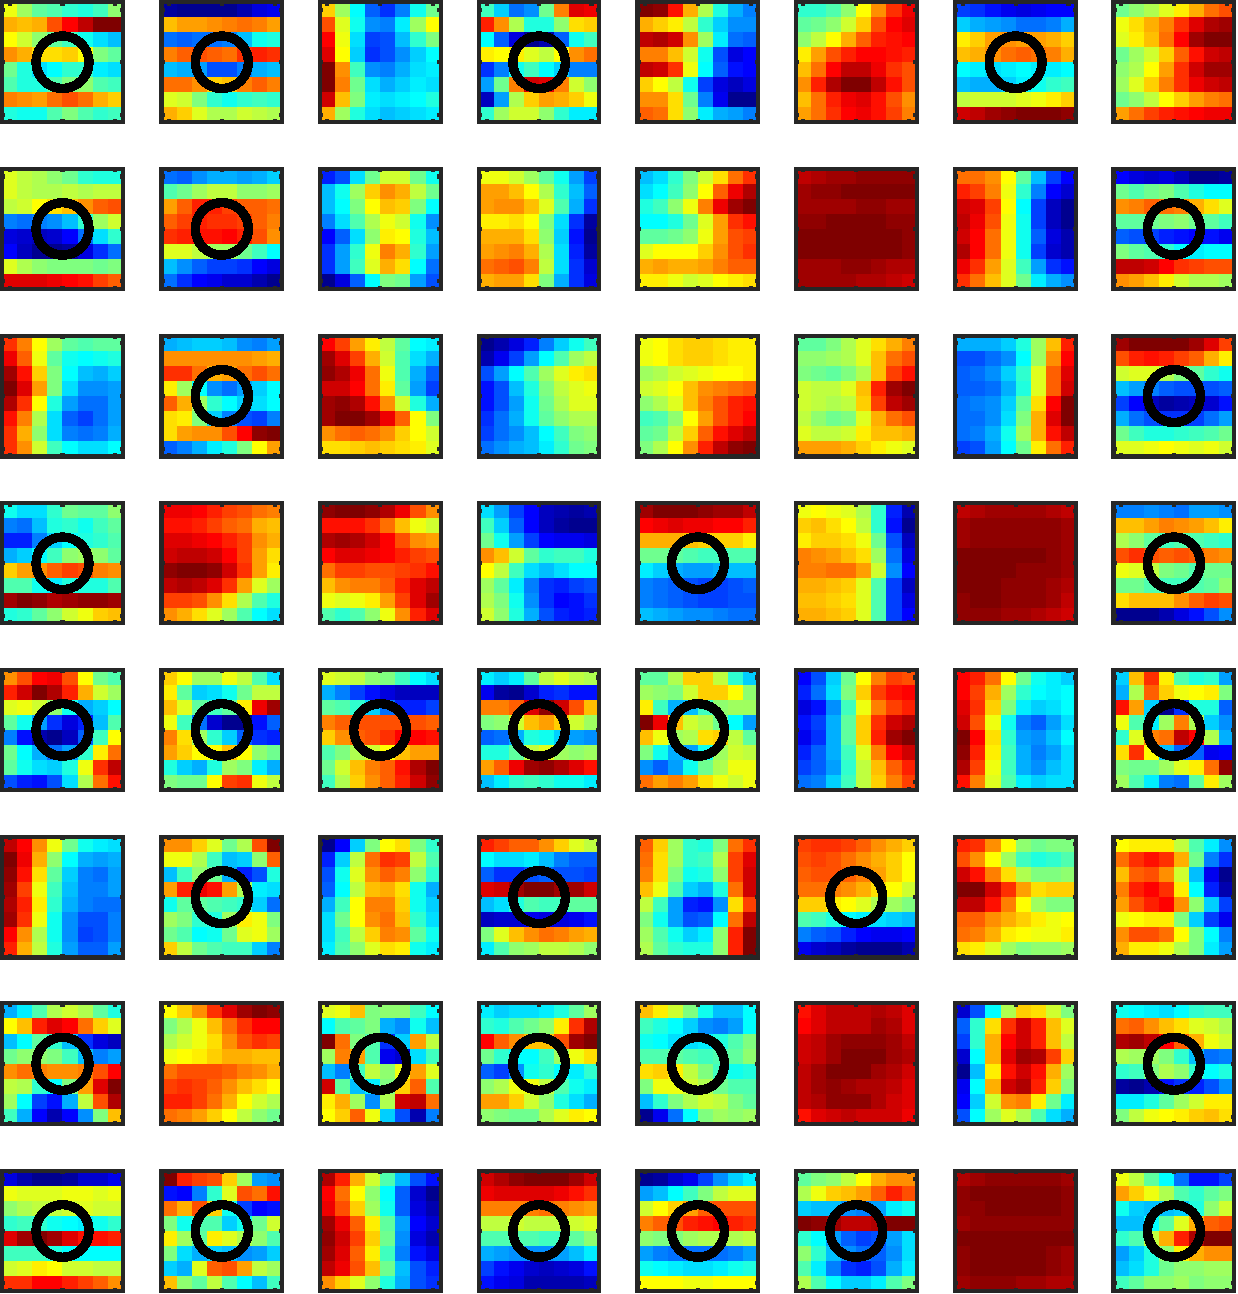
\includegraphics[width=\columnwidth]{Fig/sta_atoms2}
\caption{Learned atoms and the manual picking results. The black circle indicates that we manually define this atom as a footprint noise related atom. }
\label{fig:sta_atoms2}
\end{figure}


\begin{figure}[htb!]
\centering
\subfloat[]{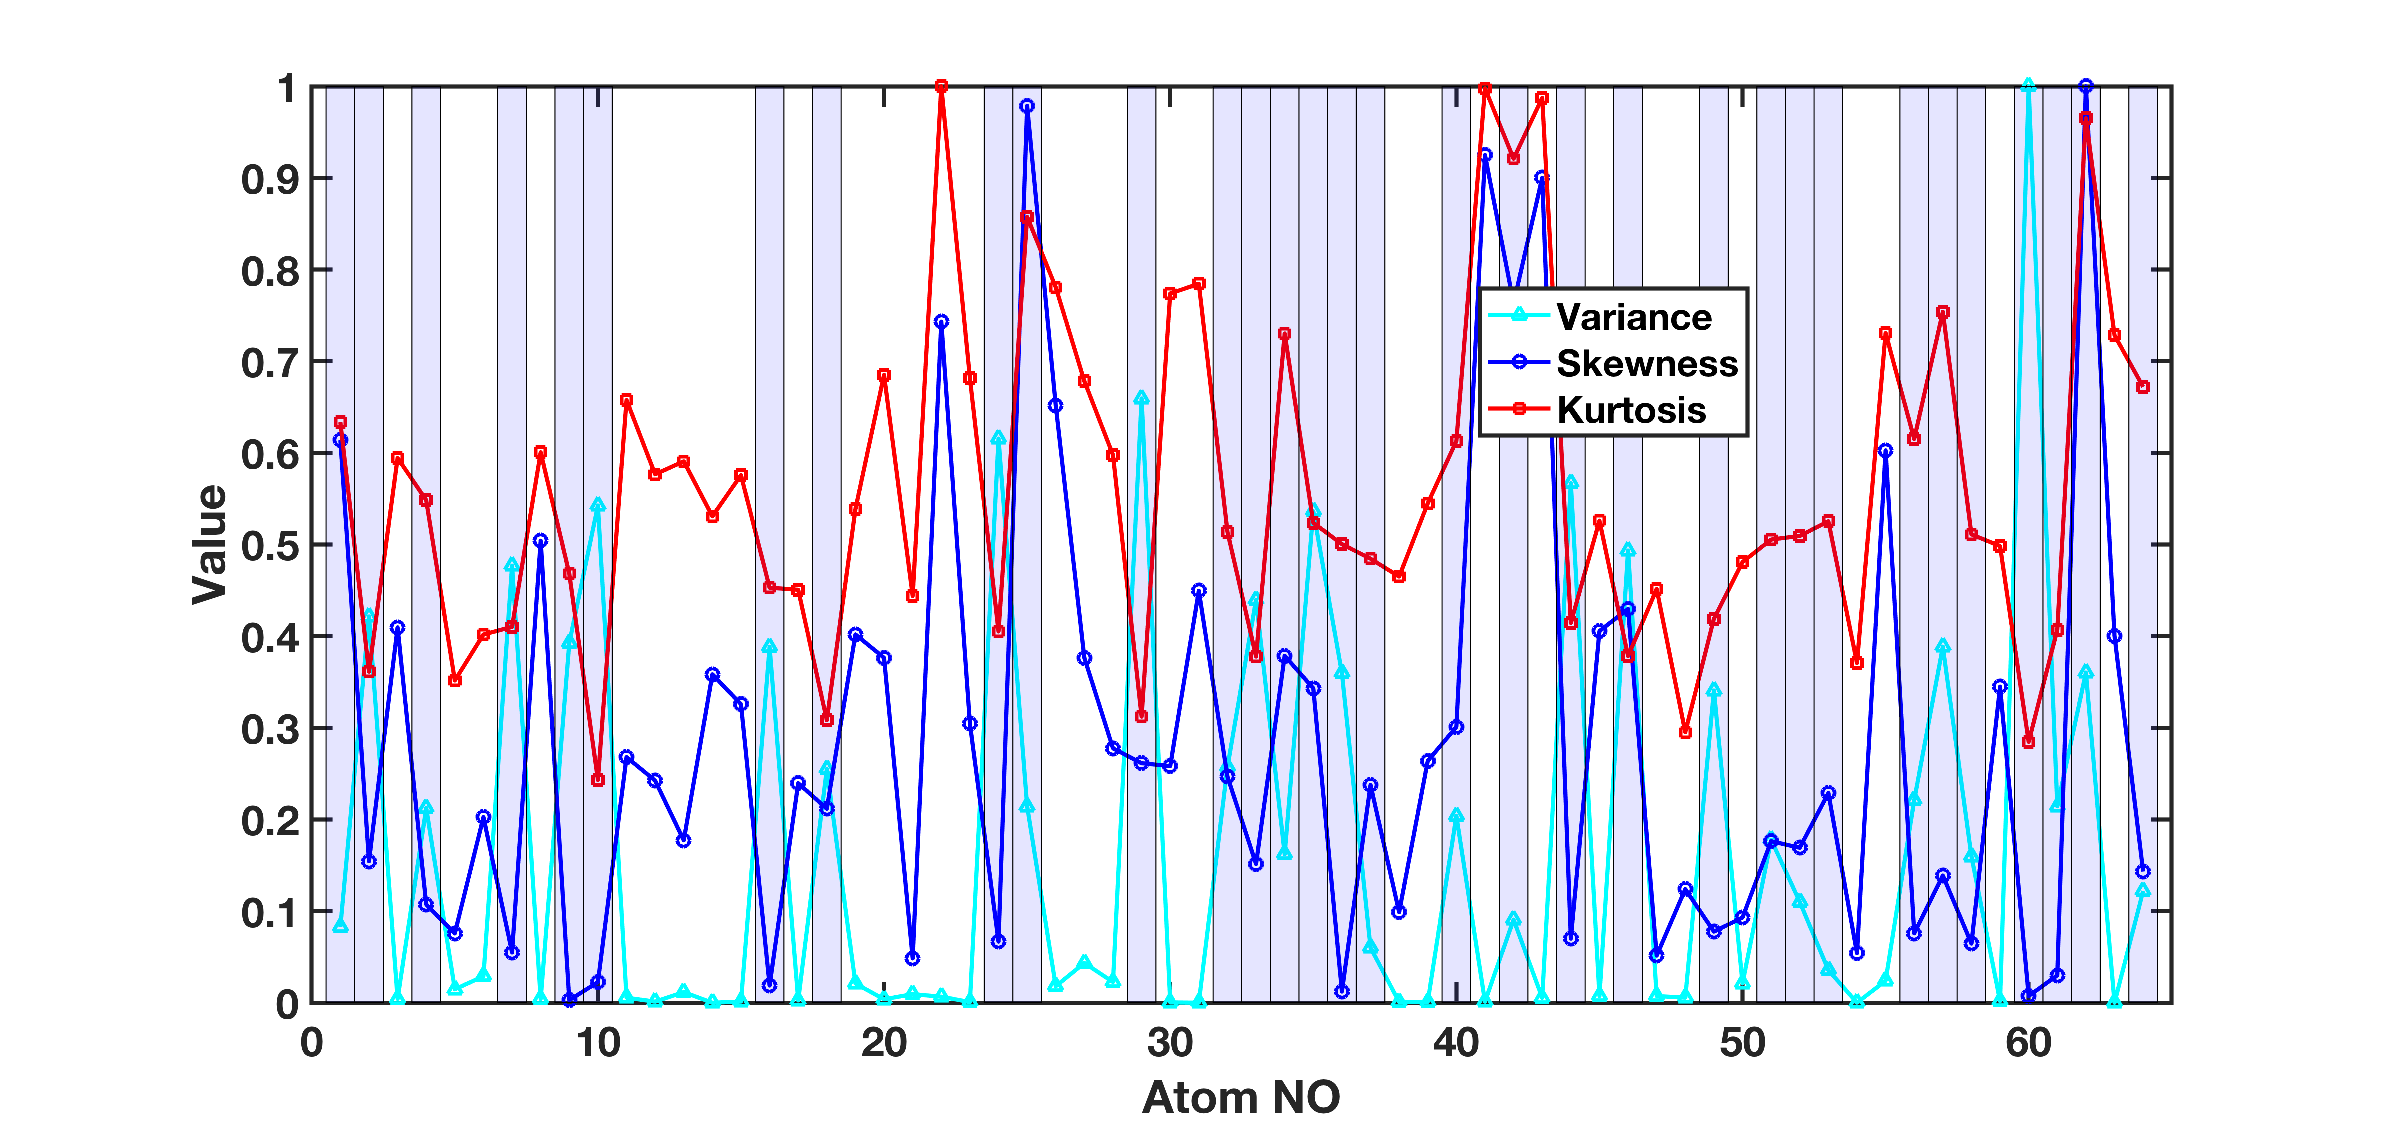
\includegraphics[width=0.8\columnwidth]{Fig/sta_curves}
   \label{fig:sta_curves}} \\
   \subfloat[]{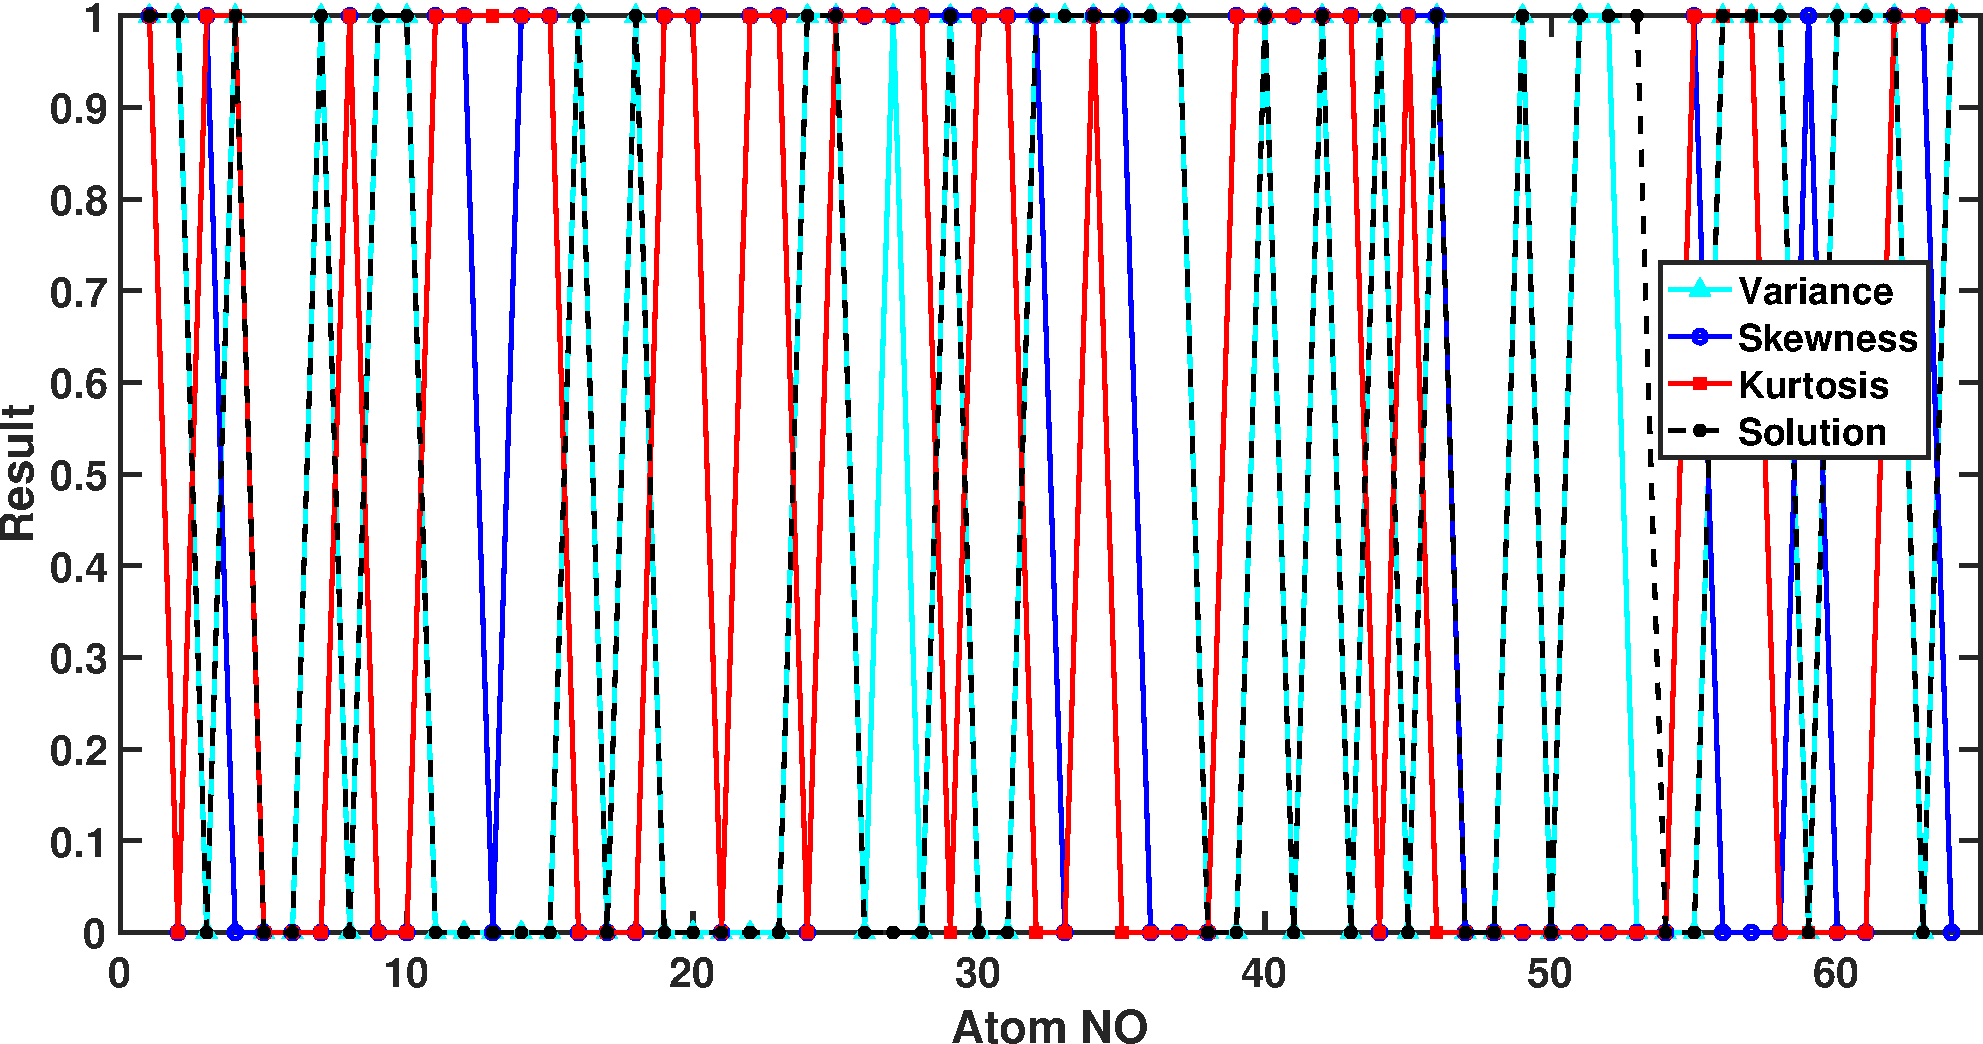
\includegraphics[width=0.7\columnwidth]{Fig/sta_result}
   \label{fig:sta_result}} \\
   \subfloat[]{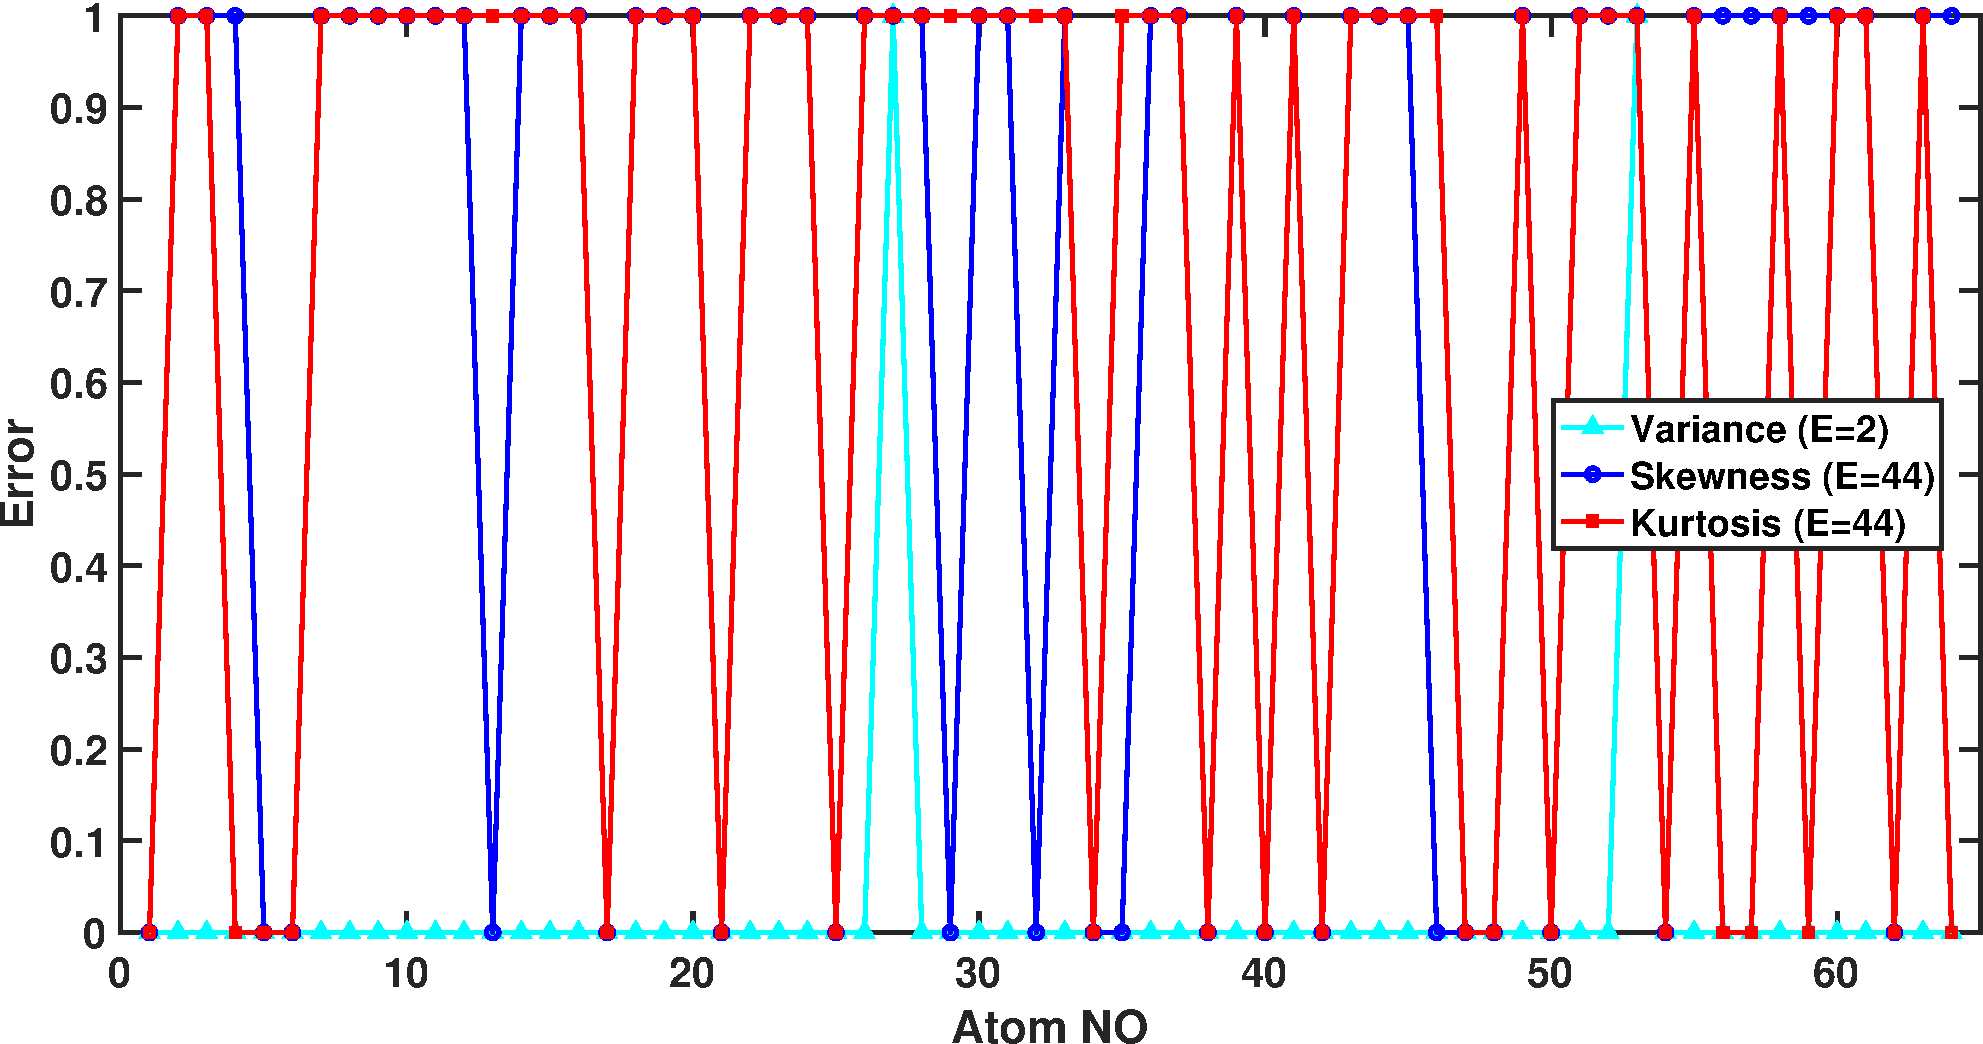
\includegraphics[width=0.7\columnwidth]{Fig/sta_err}
   \label{fig:sta_err}}
\caption{Statistic test. (a) Curves of different statistical measures. (b) Binary classification results. ``1" means noise atom and ``0" means signal atom. (c) Classification errors. Here, \new{the} error is either 1 or 0 for each atom. The summation of error $E$ of all atoms indicates the classification accuracy and is listed in the legends. }
\label{fig:sta_curves,sta_result,sta_err}
\end{figure}


\begin{figure}[htb!]
\centering
\subfloat[]{\includegraphics[width=0.32\columnwidth]{syn/Fig/syn-c}
   \label{fig:syn-c}}
\subfloat[]{\includegraphics[width=0.32\columnwidth]{syn/Fig/syn-nft}
   \label{fig:syn-nft}}\\
\subfloat[]{\includegraphics[width=0.32\columnwidth]{syn/Fig/syn-nrand}
   \label{fig:syn-nrand}}
   \subfloat[]{\includegraphics[width=0.32\columnwidth]{syn/Fig/syn-n}
   \label{fig:syn-n}}
\caption{Synthetic example. (a) Clean data. (b) Footprint noise. (c) Random noise. (d) Noisy data}
\label{fig:syn-c,syn-nft,syn-nrand,syn-n}
\end{figure}

\begin{figure}[htb!]
\centering
\subfloat[]{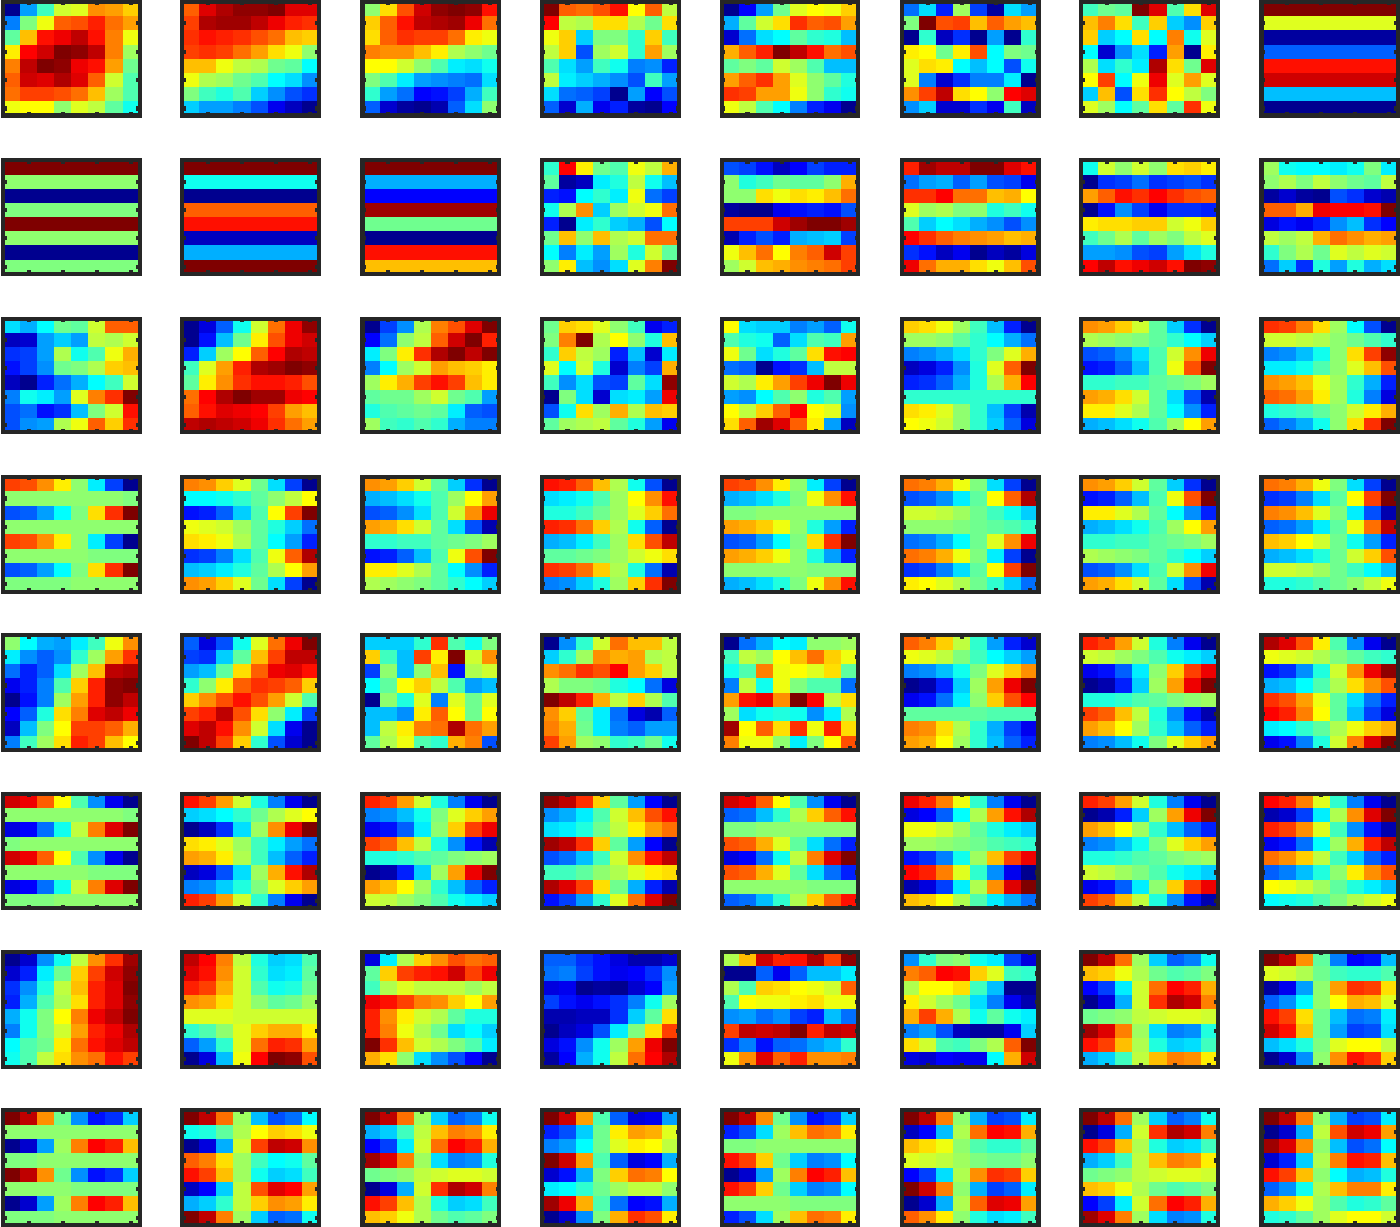
\includegraphics[width=0.45\columnwidth]{Fig/s_atom0}
   \label{fig:s_atom0}}\\
\subfloat[]{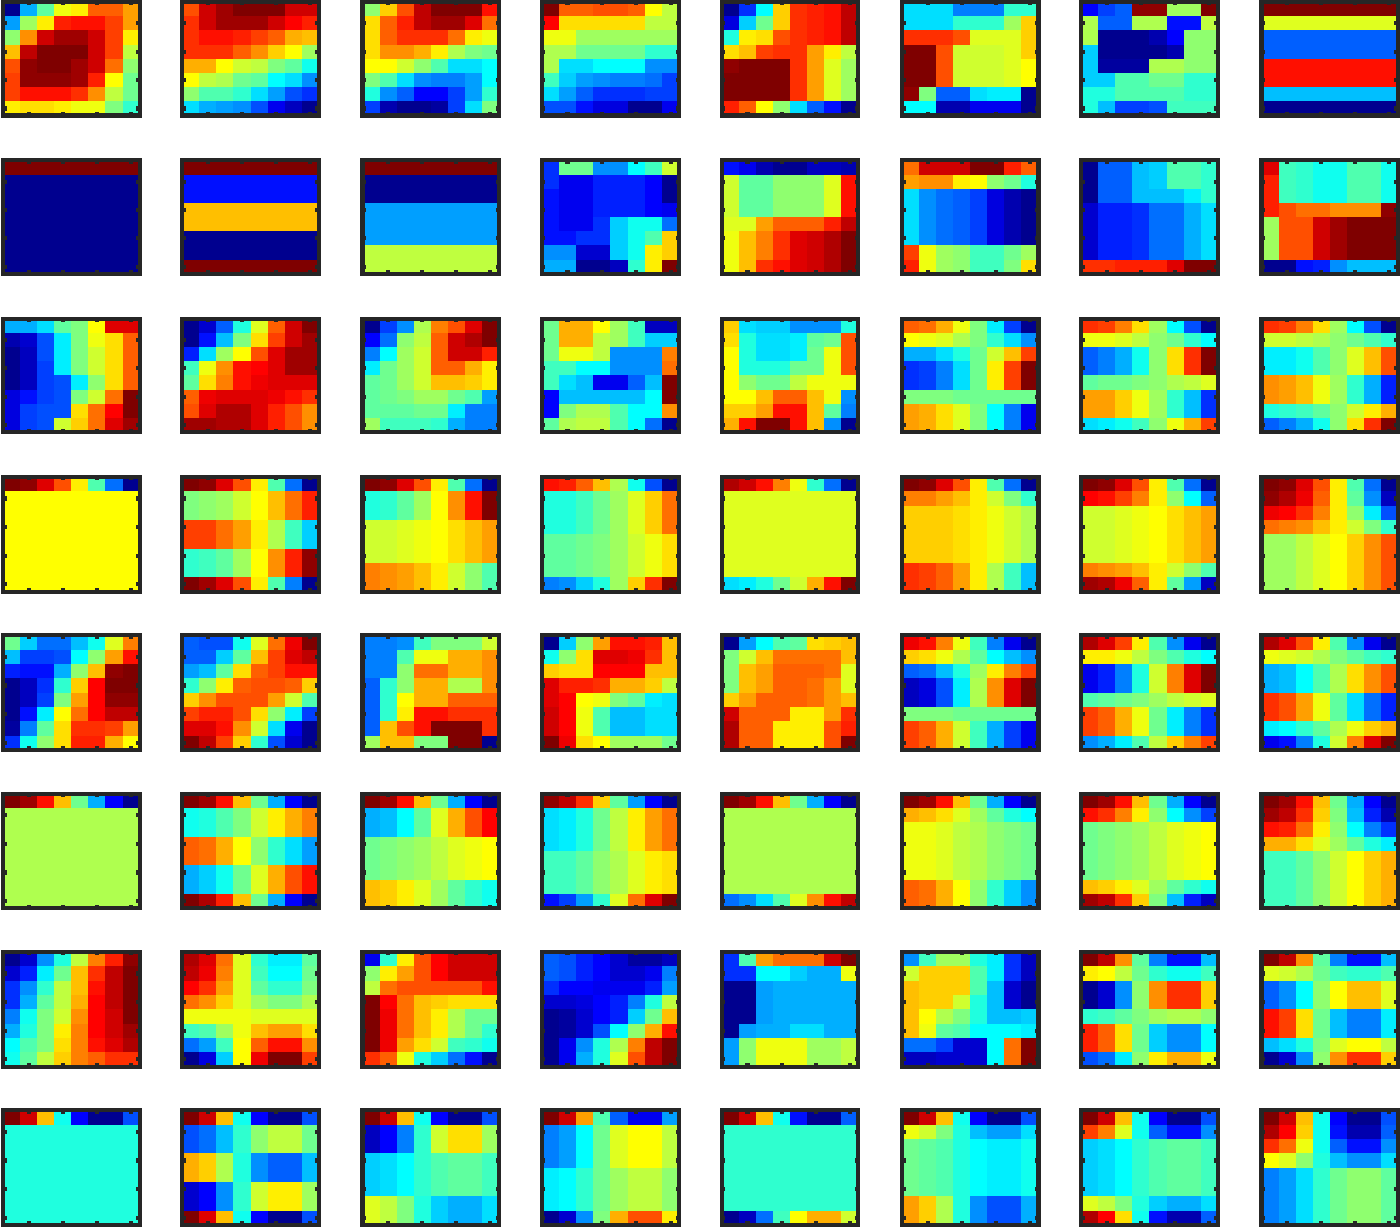
\includegraphics[width=0.45\columnwidth]{Fig/s_atom1}
   \label{fig:s_atom1}}
\subfloat[]{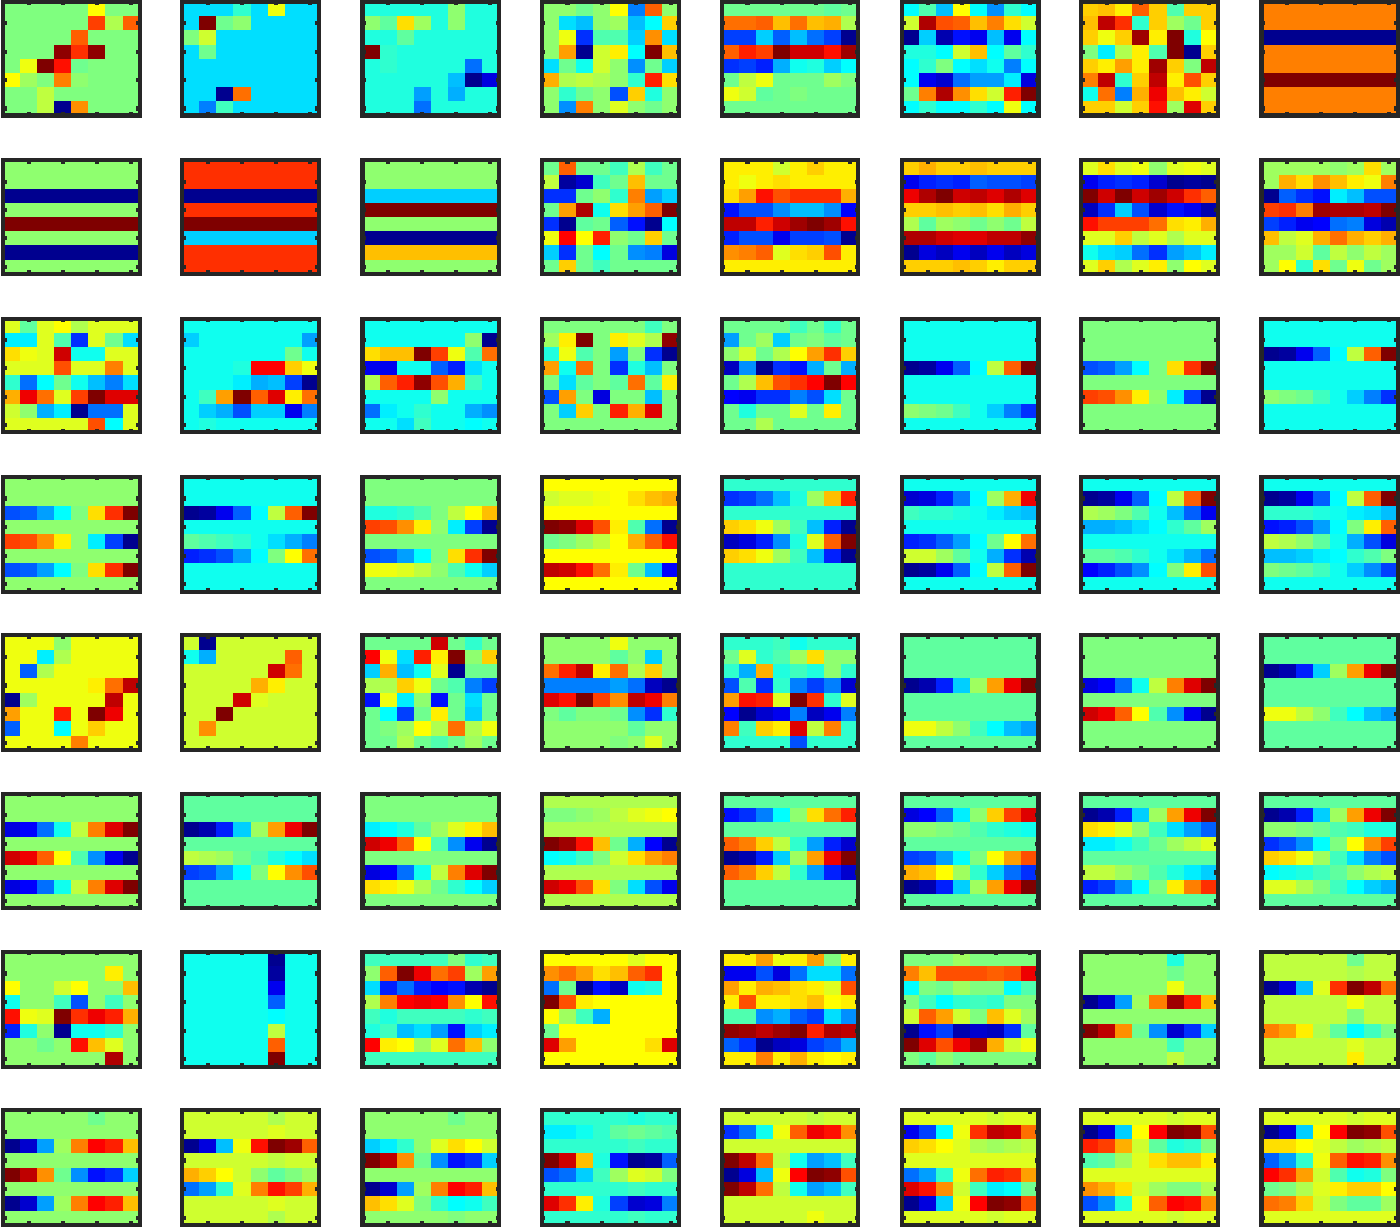
\includegraphics[width=0.45\columnwidth]{Fig/s_atom2}
   \label{fig:s_atom2}}
\caption{A comparison of the dictionary atoms of the synthetic data example. (a) Learned atoms directly from field data. (b) Learned signal atoms obtained by selecting noise-free atoms via the statistics-guided method and filtering the noise-contaminated atoms via the median filtering method. (c) Learned footprint noise atoms by subtracting (b) from (a). }
\label{fig:s_atom0,s_atom1,s_atom2}
\end{figure}

\begin{figure}[htb!]
\centering
\subfloat[]{\includegraphics[width=0.32\columnwidth]{syn/Fig/syn-drr}
   \label{fig:syn-drr}}
\subfloat[]{\includegraphics[width=0.32\columnwidth]{syn/Fig/syn-dl}
   \label{fig:syn-dl}}\\
\subfloat[]{\includegraphics[width=0.32\columnwidth]{syn/Fig/syn-mf-0}
   \label{fig:syn-mf-0}}
   \subfloat[]{\includegraphics[width=0.32\columnwidth]{syn/Fig/syn-sgrdl-0}
   \label{fig:syn-sgrdl-0}}
\caption{Denosing comparison of the synthetic example. Denoised data using (a) DRR method, (b) standard DL method, (c) median filtering method, and (d) the proposed SGRDL method. }
\label{fig:syn-drr,syn-dl,syn-mf-0,syn-sgrdl-0}
\end{figure}

\begin{figure}[htb!]
\centering
\subfloat[]{\includegraphics[width=0.32\columnwidth]{syn/Fig/syn-drr-n}
   \label{fig:syn-drr-n}}
\subfloat[]{\includegraphics[width=0.32\columnwidth]{syn/Fig/syn-dl-n}
   \label{fig:syn-dl-n}}\\
\subfloat[]{\includegraphics[width=0.32\columnwidth]{syn/Fig/syn-mf-n-0}
   \label{fig:syn-mf-n-0}}
   \subfloat[]{\includegraphics[width=0.32\columnwidth]{syn/Fig/syn-sgrdl-n-0}
   \label{fig:syn-sgrdl-n-0}}
\caption{Denosing comparison of the synthetic example. Removed noise using (a) DRR method, (b) standard DL method, (c) median filtering method, and (d) the proposed SGRDL method. }
\label{fig:syn-drr-n,syn-dl-n,syn-mf-n-0,syn-sgrdl-n-0}
\end{figure}

\begin{figure}[htb!]
\centering
\subfloat[]{\includegraphics[width=0.35\columnwidth]{syn/Fig/syn-drr-s}
   \label{fig:syn-drr-s}}
\subfloat[]{\includegraphics[width=0.35\columnwidth]{syn/Fig/syn-dl-s}
   \label{fig:syn-dl-s}}\\
\subfloat[]{\includegraphics[width=0.35\columnwidth]{syn/Fig/syn-mf-s}
   \label{fig:syn-mf-s}}
   \subfloat[]{\includegraphics[width=0.35\columnwidth]{syn/Fig/syn-sgrdl-s}
   \label{fig:syn-sgrdl-s}}
\caption{Denosing comparison of the synthetic example. Local similarity between the clean data and denoised data using (a) DRR method, (b) standard DL method, (c) median filtering method, and (d) the proposed SGRDL method. }
\label{fig:syn-drr-s,syn-dl-s,syn-mf-s,syn-sgrdl-s}
\end{figure}

\begin{figure}[htb!]
\centering
\subfloat[]{\includegraphics[width=0.3\columnwidth]{syn/Fig/syn-s-c}
   \label{fig:syn-s-c}}
\subfloat[]{\includegraphics[width=0.3\columnwidth]{syn/Fig/syn-s-n}
   \label{fig:syn-s-n}}
\subfloat[]{\includegraphics[width=0.3\columnwidth]{syn/Fig/syn-s-drr}
   \label{fig:syn-s-drr}}\\
\subfloat[]{\includegraphics[width=0.3\columnwidth]{syn/Fig/syn-s-dl}
   \label{fig:syn-s-dl}}
\subfloat[]{\includegraphics[width=0.3\columnwidth]{syn/Fig/syn-s-mf-0}
   \label{fig:syn-s-mf-0}}
\subfloat[]{\includegraphics[width=0.3\columnwidth]{syn/Fig/syn-s-sgrdl-0}
   \label{fig:syn-s-sgrdl-0}}
\caption{Single slice comparison of (a) clean data, (b) noisy data, and denoised data using (c) DRR method, (d) standard DL method, (e) median filtering method, and (f) the proposed SGRDL method. }
\label{fig:syn-s-c,syn-s-n,syn-s-drr,syn-s-dl,syn-s-mf-0,syn-s-sgrdl-0}
\end{figure}


\begin{figure}[htb!]
\centering
\subfloat[]{\includegraphics[width=0.32\columnwidth]{syn/Fig/syn-s-drr-n}
   \label{fig:syn-s-drr-n}}
\subfloat[]{\includegraphics[width=0.32\columnwidth]{syn/Fig/syn-s-dl-n}
   \label{fig:syn-s-dl-n}}\\
\subfloat[]{\includegraphics[width=0.32\columnwidth]{syn/Fig/syn-s-mf-n-0}
   \label{fig:syn-s-mf-n-0}}
\subfloat[]{\includegraphics[width=0.32\columnwidth]{syn/Fig/syn-s-sgrdl-n}
   \label{fig:syn-s-sgrdl-n}}
\caption{Single slice comparison of removed noise using (a) DRR method, (b) standard DL method, (c) median filtering method, and (d) the proposed SGRDL method. }
\label{fig:syn-s-c,syn-s-n,syn-s-drr,syn-s-dl,syn-s-mf-0,syn-s-sgrdl}
\end{figure}



\begin{figure}[htb!]
\centering
\subfloat[]{\includegraphics[width=0.3\columnwidth]{syn/Fig/syn-c-t}
   \label{fig:syn-c-t}}
\subfloat[]{\includegraphics[width=0.3\columnwidth]{syn/Fig/syn-n-t}
   \label{fig:syn-n-t}}
\subfloat[]{\includegraphics[width=0.3\columnwidth]{syn/Fig/syn-drr-t}
   \label{fig:syn-drr-t}}\\
\subfloat[]{\includegraphics[width=0.3\columnwidth]{syn/Fig/syn-dl-t}
   \label{fig:syn-dl-t}}
\subfloat[]{\includegraphics[width=0.3\columnwidth]{syn/Fig/syn-mf-t}
   \label{fig:syn-mf-t}}
\subfloat[]{\includegraphics[width=0.3\columnwidth]{syn/Fig/syn-sgrdl-t}
   \label{fig:syn-sgrdl-t}}
\caption{Single slice comparison of (a) clean data, (b) noisy data, and denoised data using (c) DRR method, (d) standard DL method, (e) median filtering method, and (d) the proposed SGRDL method. }
\label{fig:syn-c-t,syn-n-t,syn-drr-t,syn-dl-t,syn-mf-t,syn-sgrdl-t}
\end{figure}

\begin{figure}[htb!]
\centering
\subfloat[]{\includegraphics[width=\columnwidth]{syn/Fig/syn-ss-0}
   \label{fig:syn-ss-0}}\\
\subfloat[]{\includegraphics[width=\columnwidth]{syn/Fig/syn-ss-z}
   \label{fig:syn-ss-z}}
\caption{Single trace comparison. The black line corresponds to the clean data. The green line corresponds to the noisy data. The red line corresponds to the proposed SGRDL method. The magenta line corresponds to the MF method. The blue line corresponds to the standard DL method. The cyan line corresponds to the DRR method. (a) Comparison in the original scale. (b) Comparison in the zoomed scale. It is clear from (b) that the red line is the closest to the ground-truth solution (the black line). }
\label{fig:syn-ss-0,syn-ss-z}
\end{figure}

\subsection{Statistics guided dictionary atom filtering}
When seismic data contain footprint noise, the learned dictionary atoms have special features. It is possible to manually pick those atoms that correspond to signals, e.g., in \cite{liu2020deep}. However, it is more convenient to develop an automatic way to classify the atoms into noise-contaminated and the noise-free atoms.  Here, we propose a statistics guided method for this task, like the one in \cite{yatong2021}. Since the footprint noise is a type of coherent noise, and appears as coherent stripes in the atoms, we propose to leverage several 2D statistical metrics to distinguish between disparate atoms. 


Supposing each atom is of size ($l_1l_2\times 1$), for calculating the 2D statistical metrics, we first reshape each atom into a rectangle $A(i,j)$ of size $l_1\times l_2$. According to the shape of the footprint noise, e.g., horizontal or vertical, the statistical metrics are calculated along each column or row of the rectangle $A(i,j)$. Let us take the horizontal footprint noise as an example. The statistic metrics are calculated along the vertical direction of the rectangle $A(i,j)$:
\begin{equation}
\label{eq:me}
y=\sum_{j=1}^{l_2} f(\mathbf{a}_j),
\end{equation}
where $y$ is the output 2D statistic metric. $f(\cdot)$ denotes a 1D statistical metric, e.g., variance, skewness, and kurtosis, while $\mathbf{a}_j$ denotes the $j$th column in the rectangle $A(i,j)$. Here, we list three 1D statistical metrics as follows:
\begin{enumerate}
\item Variance
\begin{equation}
\label{eq:v}
v(\mathbf{a}) = \frac{1}{l_1} \sum_{i=1}^{l_1} [a(i) - \mu]^2,
\end{equation}
where $\mu= | \frac{1}{l_1} \sum_{i=1}^{l_1} a(i) |$ denotes the mean of the input vector $\mathbf{a}$. $a(i)$ denotes the $i$th entry in vector $\mathbf{a}$. 


\item Skewness
\begin{equation}
\label{eq:s}
s(\mathbf{a})= \frac{ \displaystyle \frac{1}{l_1} \sum_{i=1}^{l_1} [a(i)-\mu]^3}{\displaystyle \left(\frac{1}{l_1}\left(\sum_{i=1}^{l_1} [a(i)-\mu]^2\right)\right)^{3/2} }.
\end{equation}

\item Kurtosis
\begin{equation}
\label{eq:k}
k(\mathbf{a}) = \frac{ \displaystyle \frac{1}{l_1} \sum_{i=1}^{l_1} [a(i)-\mu]^4}{\displaystyle \left(\frac{1}{l_1}\left(\sum_{i=1}^{l_1} [a(i)-\mu]^2\right)\right)^2 }.
\end{equation}
\end{enumerate}



To compare the effectiveness of different metrics in distinguishing between the noise-contaminated and noise-free atoms, we show some typical atoms extracted from a field dataset that are contaminated by footprint noise in Figure \ref{fig:sta_atoms2}. Each atom has a size of $8\times 8$. It is clear that among the 64 atoms, the morphological features can be roughly divided into two types, i.e., \old{wether}\new{whether} containing horizontal stripes or not. It is easy to pick those stripes-contaminated atoms manually from the 64 atoms, as indicated by the black circles in the middle of each atom. In this example, we manually choose 32 noise-contaminated atoms with the others being the noise-free atoms. The noise-contaminated atoms need to be filtered out in order to better represent the useful signal via the sparse coding process. To see which statistical metric best detects the morphological anomalies shown in the noise-contaminated atoms, we calculate the aforementioned statistical metrics for all these atoms. We show the values of different statistical metrics for all 64 atoms in Figure \ref{fig:sta_curves}. Red, blue, cyan correspond to kurtosis, skewness, and variance, respectively. We also plot the manually picked noise-contaminated atoms as the light blue windows overlapping the curves in Figure \ref{fig:sta_curves}. It is clear that the abnormally high values of the variance curve correlate with the existence of light windows well. However, the red kurtosis curve and blue skewness curve do not show clear correlation patterns. 

We use these statistical metrics as the criterion for a binary classification, i.e., 1 for noise-contaminated atoms and 0 for noise-free atoms. We plot the classification results of different statistical metrics and the ground-truth solution (defined by the manual picks) in Figure \ref{fig:sta_result}. \new{It is clear that the curve using the variance metric is mostly overlapping the ground-truth solution, indicating a very accurate classification performance. The kurtosis (red) and skewness (blue) metrics, however, deviate greatly from the ground-truth solution.} Figure \ref{fig:sta_err} plots the errors using the three statistical metrics. It is clear that the error of the variance metric is mostly zero while the other two metrics cause significant classification error. Here, the error in the classification is defined as \cite{yangkang2018gji}:
\begin{equation}
\label{eq:err}
\text{E} = \sum_{i=1}^{K} |I(i) - \hat{I}(i) |,
\end{equation}
where $i$ denotes the atom index, $I$ denotes the classification result (1 or 0) for the ground-truth solution, $\hat{I}$ is the classification output using different methods. The error corresponding to the variance metric is only 2,  meaning that only two atoms are not classified correctly, while the errors of the kurtosis and skewness metrics are both 44, meaning that 44 atoms (in 64) are classified inaccurately.  Thus, we use the variance metric as the criterion to divide the learned atoms into noise-free and noise-contaminated atoms. 

The noise-contaminated atoms, however, are not simply deserted. Since these atoms may still contain significant signal features that are hidden in the stripes-like noise, we propose to apply a median filter along the vertical direction to filter out stripes-like noise and recover the signal features. We obtain the signal atoms by combining the noise-free atoms picked by the statistic-guided method and the filtered noise-contaminated atoms via median filtering. In cases that the picked noise-free atoms still contain very weak stripes-like noise features, they will be processed by a weak median filters to further filter out the noise features. 
After the filtering, we obtain two dictionaries, i.e., signal and noise dictionaries. 
%% also add an algorithm 

\subsection{Residual dictionary learning}
Supposing the filtered dictionary is $\tilde{\mathbf{D}}$,  in a traditional sparse coding method, the denoised seismic data can be obtained by \old{first }sparse coding:
\begin{equation}
\label{eq:sc0}
\forall_i \tilde{\mathbf{m}}_{i}=\arg\min_{\mathbf{M}}||\mathbf{Y}-\tilde{\mathbf{D}}\mathbf{M}||^{2}_{F}, \quad\text{s.t.}  \quad \forall_i ||\mathbf{m}_{i}||_{0}\le Q,
\end{equation}
\old{then, by linear combination of the learned dictionary atoms based on the sparse coefficients. We can obtain the denoised data using a standard dictionary learning scheme:}\new{then, by linear combination of the learned dictionary atoms based on the sparse coefficients, we can obtain the denoised data using a standard dictionary learning scheme:}
\begin{equation}
\label{eq:sc1}
\tilde{\mathbf{Y}} = \tilde{\mathbf{D}} \tilde{\mathbf{M}},
\end{equation}
where $\tilde{\mathbf{M}}$ is composed \old{by}\new{of} $\tilde{\mathbf{m}}_{i}$, and $\tilde{\mathbf{Y}}$ denotes the denoised patches.

In the proposed method, to make the denoised data $\tilde{\mathbf{D}}$ less contaminated by the footprint noise, we propose the following augmented sparse coding problem:
\begin{equation}
\label{eq:sc2}
\begin{split}
\forall_i [\tilde{\mathbf{m}}_{i},\tilde{\mathbf{g}}_{i}]&=\arg\min||\mathbf{Y}-\tilde{\mathbf{D}}\mathbf{M} - \tilde{\mathbf{B}}\mathbf{G} ||^{2}_{F}, \\
& \quad\text{s.t.}  \quad \forall_i ||\mathbf{m}_{i}||_{0}+||\mathbf{g}_{i}||_{0} \le Q,
\end{split}
\end{equation}
where $\tilde{\mathbf{B}}$ denotes the learned footprint feature atoms. It can be calculated simply by
\begin{equation}
\label{eq:ftf}
\tilde{\mathbf{B}}=\mathbf{D}-\tilde{\mathbf{D}}.
\end{equation}
Equation \ref{eq:sc2} is equivalent to learning the residual of the traditional dictionary learning $\mathbf{R}=\mathbf{Y}-\tilde{\mathbf{D}}\mathbf{M}$ via the learned footprint feature atoms $\tilde{\mathbf{B}}$. Thus, we call it residual dictionary learning.

%Let $\overline{\mathbf{D}} = [\tilde{\mathbf{D}},\tilde{\mathbf{B}}]$, and 
Equation \ref{eq:sc2} can be expressed as:
\begin{equation}
\label{eq:sc22}
\forall_i \tilde{\mathbf{p}}_{i}=\arg\min||\mathbf{Y}-\mathbf{F}\mathbf{P} ||^{2}_{F}, \quad\text{s.t.}  \quad \forall_i ||\mathbf{p}_{i}||_{0} \le Q,
\end{equation}
where 
\begin{equation}
\label{eq:scF}
\mathbf{F} = \left[\begin{array}{cc}
\tilde{\mathbf{D}} & \tilde{\mathbf{B}}
\end{array}
\right], \text{and}, 
\mathbf{P} = \left[\begin{array}{c}
\mathbf{M} \\
\mathbf{G}
\end{array}
\right].
\end{equation}
Equation \ref{eq:sc2} can be solved via the standard OMP algorithm. The solution of equation \ref{eq:sc2} ($\tilde{\mathbf{P}}$) can be expressed as:
\begin{equation}
\label{eq:scF}
\tilde{\mathbf{P}} = \left[\begin{array}{c}
\tilde{\mathbf{M}} \\
\tilde{\mathbf{G}}
\end{array}
\right],
\end{equation}
where $\tilde{\mathbf{M}}$ and $\tilde{\mathbf{G}}$ denote the sparse coefficients corresponding to the signal atoms $\tilde{\mathbf{D}}$ and noise atoms $\tilde{\mathbf{B}}$. The denoised data $\tilde{\mathbf{S}}$ and estimated footprint noise $\tilde{\mathbf{N}}$ can be represented by:
\new{\begin{equation}
\label{eq:sc1}
\tilde{\mathbf{S}} = \tilde{\mathbf{D}} \tilde{\mathbf{M}}\quad \text{and} \quad
\tilde{\mathbf{N}} = \tilde{\mathbf{B}} \tilde{\mathbf{G}}.
\end{equation}}

The complete algorithm of the proposed statistics-guided residual dictionary learning method (SGRDL) is detailed in Algorithm \ref{alg:alg1}.

\begin{algorithm}[htb!]
   \caption{Statistics-guided residual dictionary learning algorithm}
   \textbf{Input:} Noisy data $\mathbf{d}$, number of learning iterations $N_{iter}$, sparsity parameter $Q$.
    \begin{algorithmic}[1]
    \State Segment the data using a patching scheme
        \For{$i$ = $1,\cdots,N_{iter}$}
     \State \textbf{Solve}: $\hat{\mathbf{D}}^n = \arg\min_{\mathbf{D}^n} \parallel \mathbf{Y} - \mathbf{D}^n\mathbf{M}^n \parallel_F^2$
     \State \textbf{Solve}: $\hat{\mathbf{M}}^n = \arg\min_{\mathbf{M}^n} \parallel \mathbf{Y} - \mathbf{D}^n\mathbf{M}^n \parallel_F^2, \quad\text{s.t.}  \quad \forall_i ||\mathbf{m}_{i}||_{0}\le Q$
        \EndFor 
        \State Atom classification based on the statistics-guided scheme
        \State Apply median filtering to noise-contaminated atoms
        \State Augment the dictionary by $\mathbf{F} = [\tilde{\mathbf{D}}, \tilde{\mathbf{B}}]$
        \State Sparse coding by solving: $\forall_i [\tilde{\mathbf{p}}_{i}]=\arg\min_{\mathbf{P}}||\mathbf{Y}-\mathbf{F}\mathbf{P} ||^{2}_{F}, \quad\text{s.t.}  \quad \forall_i ||\mathbf{p}_{i}||_{0} \le Q$
        \State Obtain the denoised patches $\tilde{\mathbf{S}} = \tilde{\mathbf{D}} \tilde{\mathbf{M}}$
        \State Reconstruct the data via an unpatching scheme
%         \State \textbf{1D inverse FFT}: $\hat{D}(x,t)=\text{IFFT}\left(\hat{D}(x,w)\right)$
\end{algorithmic}
   \textbf{Output:} Denoised data $\hat{\mathbf{d}}$
\label{alg:alg1}
\end{algorithm}





\begin{figure}[htb!]
\centering
\subfloat[]{\includegraphics[width=0.8\columnwidth]{peno/Fig/p}}
\caption{3D field data (the Penobscot dataset). }
\label{fig:p}
\end{figure}

\begin{figure}[htb!]
\centering
\subfloat[]{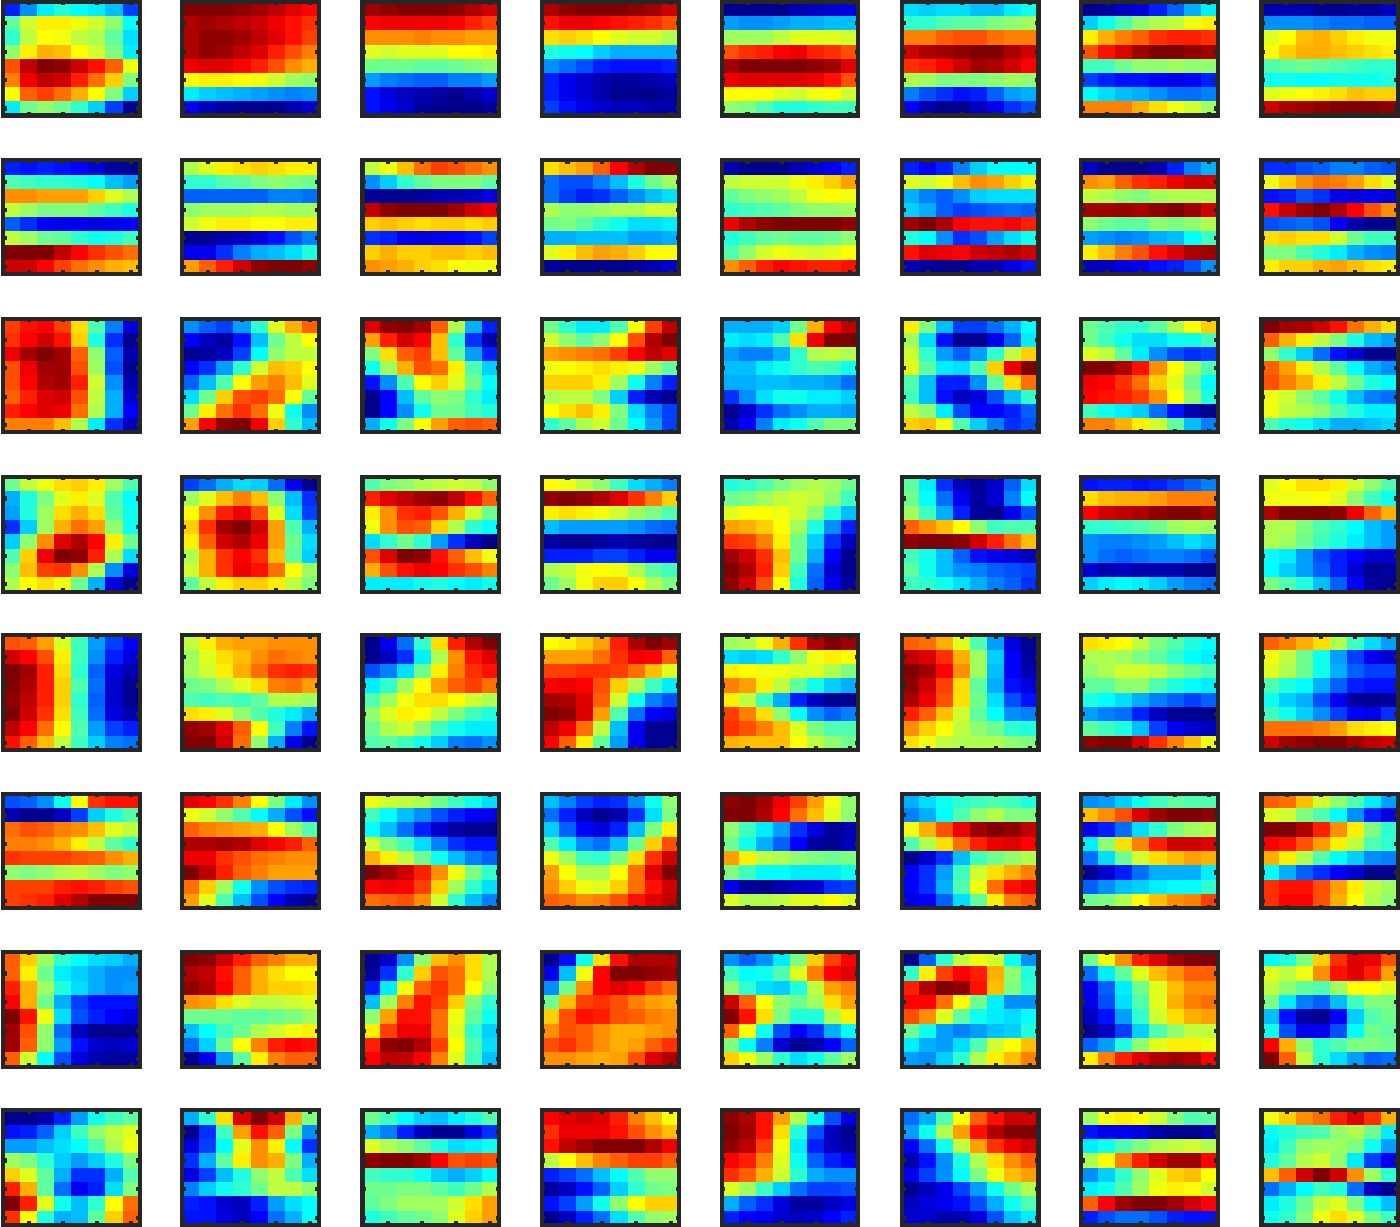
\includegraphics[width=0.45\columnwidth]{Fig/p_atom0}
   \label{fig:p_atom0}}\\
\subfloat[]{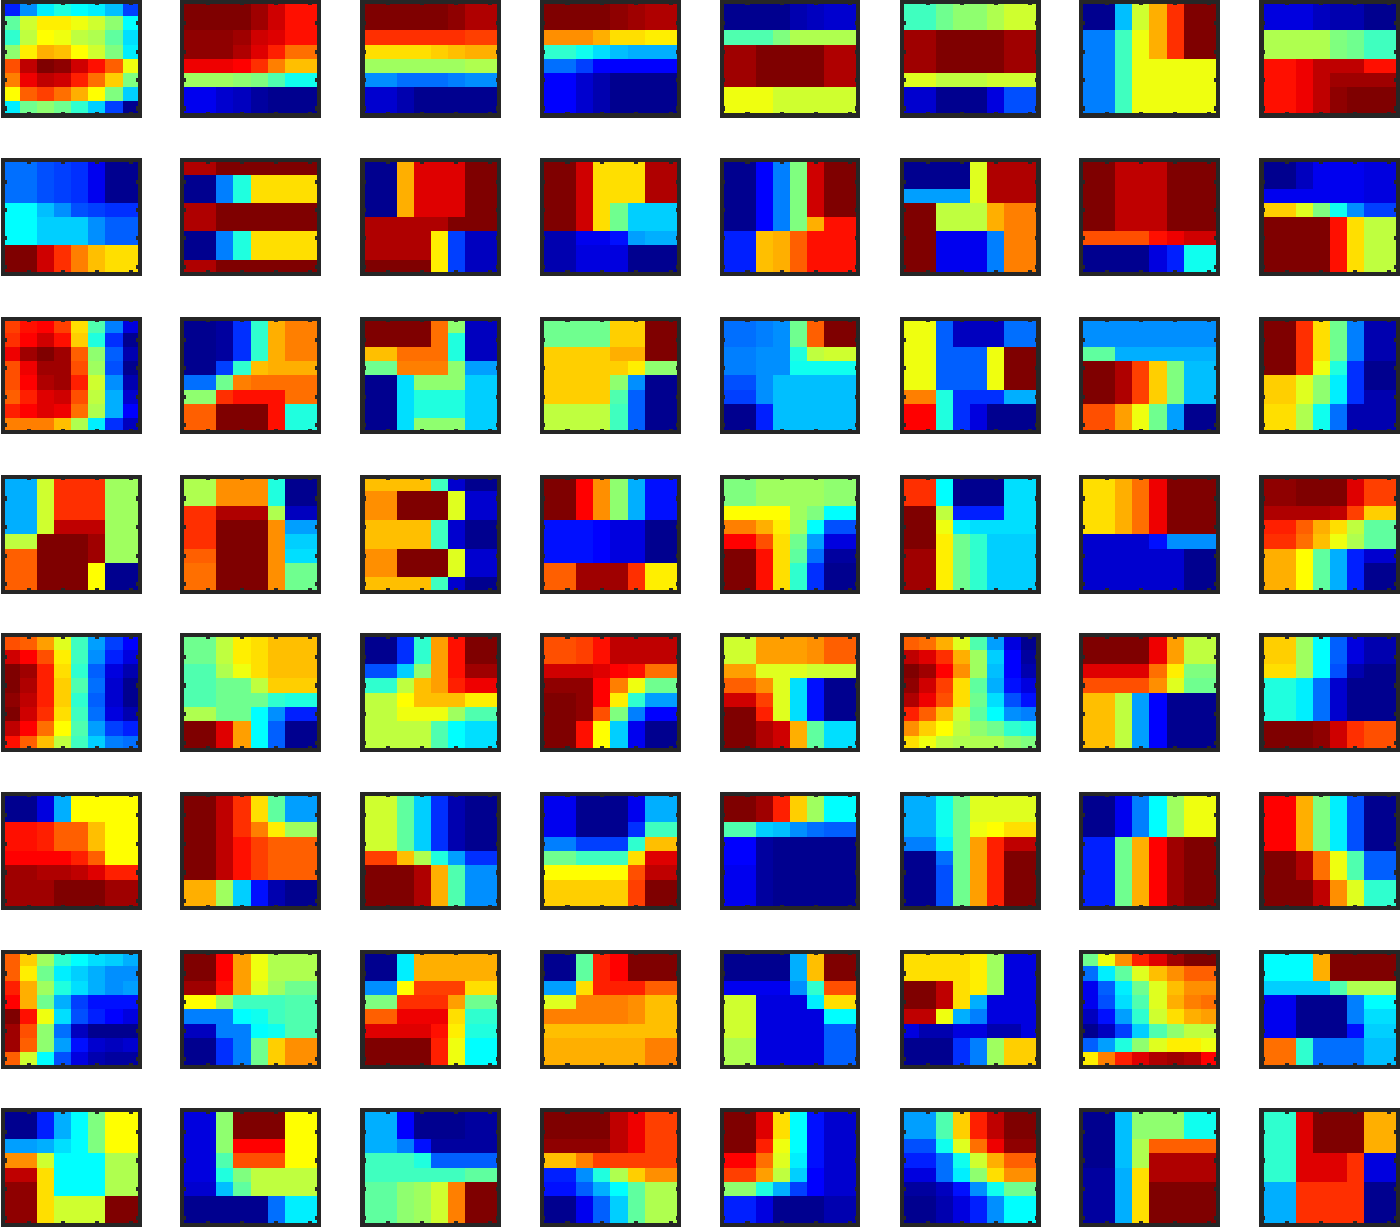
\includegraphics[width=0.45\columnwidth]{Fig/p_atom1}
   \label{fig:p_atom1}}
\subfloat[]{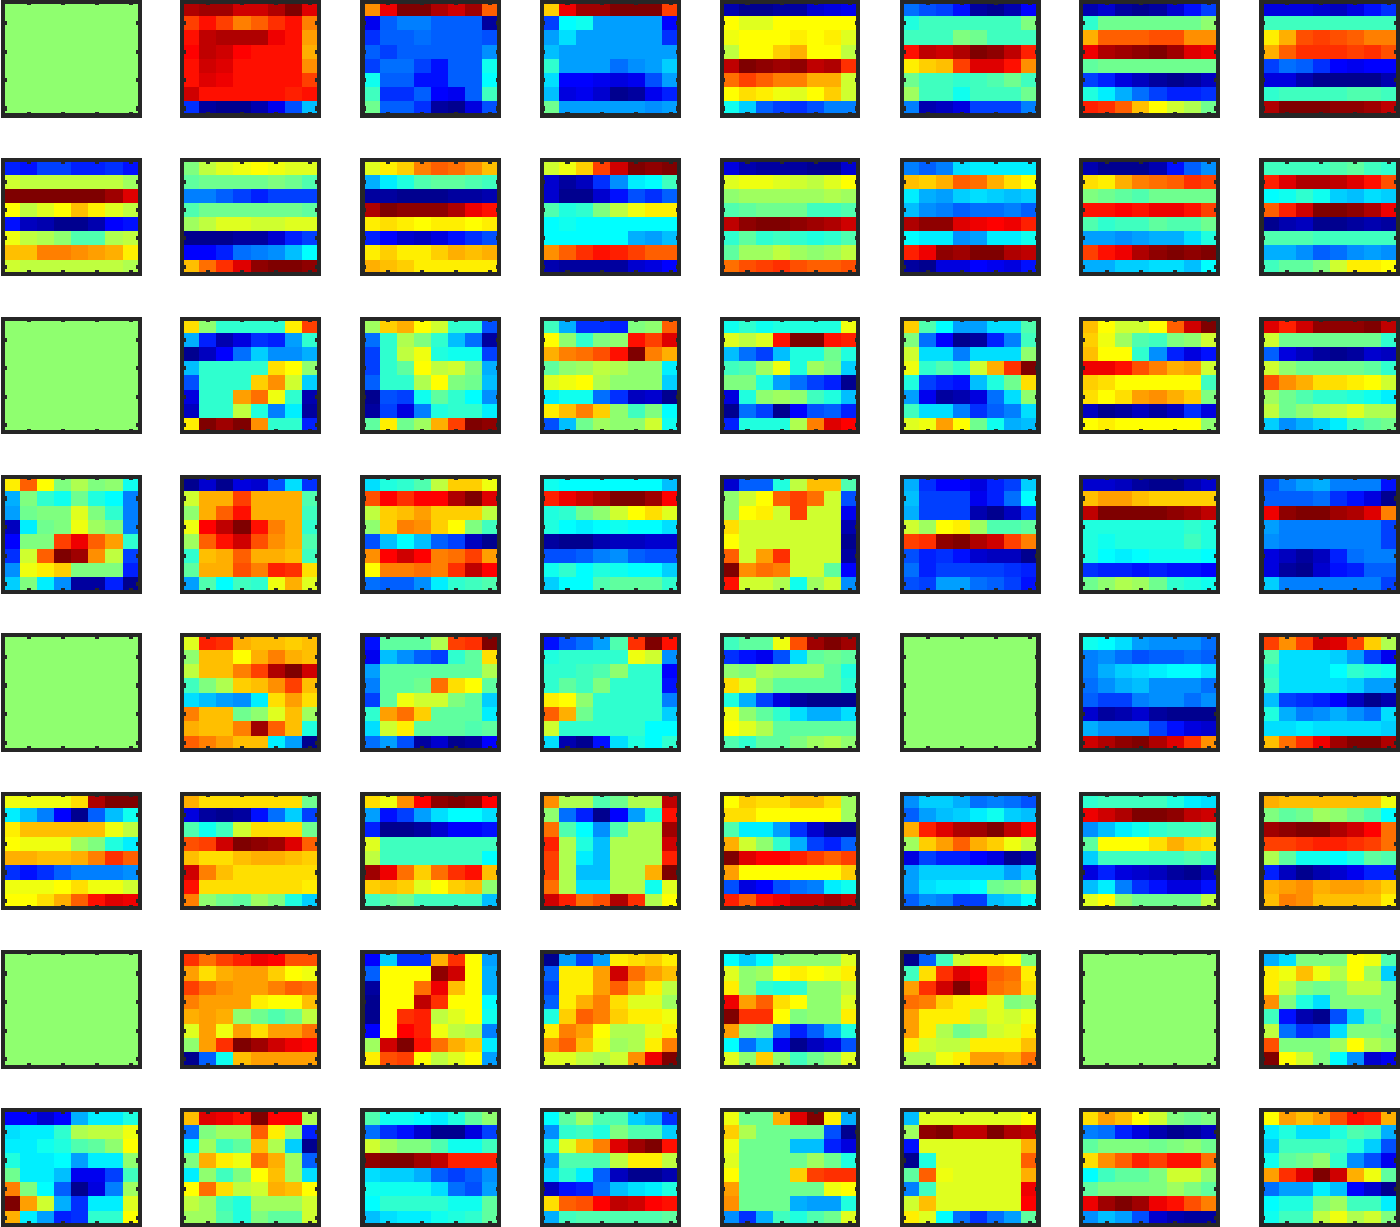
\includegraphics[width=0.45\columnwidth]{Fig/p_atom2}
   \label{fig:p_atom2}}
\caption{A comparison of the dictionary atoms of the field data example. (a) Learned atoms directly from field data. (b) Learned signal atoms obtained by selecting noise-free atoms via the statistics-guided method and filtering the noise-contaminated atoms via the median filtering method. (c) Learned footprint noise atoms by subtracting (b) from (a). The green atoms indicate those selected noise-free atoms. }
\label{fig:p_atom0,p_atom1,p_atom2}
\end{figure}

\begin{figure}[htb!]
\centering
\subfloat[]{\includegraphics[width=0.45\columnwidth]{peno/Fig/p-drr}
   \label{fig:p-drr}}
\subfloat[]{\includegraphics[width=0.45\columnwidth]{peno/Fig/p-dl-0}
   \label{fig:p-dl-0}}\\
\subfloat[]{\includegraphics[width=0.45\columnwidth]{peno/Fig/p-mf}
   \label{fig:p-mf}}
   \subfloat[]{\includegraphics[width=0.45\columnwidth]{peno/Fig/p-sgrdl}
   \label{fig:p-sgrdl}}
\caption{Denosing comparison of the field data example. Denoised data using (a) DRR method, (b) standard DL method, (c) median filtering method, and (d) the proposed SGRDL method. }
\label{fig:p-drr,p-dl-0,p-mf,p-sgrdl}
\end{figure}

\begin{figure}[htb!]
\centering
\subfloat[]{\includegraphics[width=0.45\columnwidth]{peno/Fig/p-drr-n-0}
   \label{fig:p-drr-n-0}}
\subfloat[]{\includegraphics[width=0.45\columnwidth]{peno/Fig/p-dl-n}
   \label{fig:p-dl-n}}\\
\subfloat[]{\includegraphics[width=0.45\columnwidth]{peno/Fig/p-mf-n-0}
   \label{fig:p-mf-n-0}}
   \subfloat[]{\includegraphics[width=0.45\columnwidth]{peno/Fig/p-sgrdl-n}
   \label{fig:p-sgrdl-n}}
\caption{Denosing comparison of the field data example. Removed noise using (a) DRR method, (b) standard DL method, (c) median filtering method, and (d) the proposed SGRDL method. }
\label{fig:p-drr-n-0,p-dl-n,p-mf-n-0,p-sgrdl-n}
\end{figure}



\begin{figure}[htb!]
\centering
\subfloat[]{\includegraphics[width=0.45\columnwidth]{peno/Fig/p-t}
   \label{fig:p-t}}\\
\subfloat[]{\includegraphics[width=0.45\columnwidth]{peno/Fig/p-drr-t}
   \label{fig:p-drr-t}}
\subfloat[]{\includegraphics[width=0.45\columnwidth]{peno/Fig/p-dl-t}
   \label{fig:p-dl-t}}\\
\subfloat[]{\includegraphics[width=0.45\columnwidth]{peno/Fig/p-mf-t}
   \label{fig:p-mf-t}}
   \subfloat[]{\includegraphics[width=0.45\columnwidth]{peno/Fig/p-sgrdl-t}
   \label{fig:p-sgrdl-t}}
\caption{Constant time slice comparison of the field data example. Denoised data using (a) DRR method, (b) standard DL method, (c) median filtering method, and (d) the proposed SGRDL method. }
\label{fig:p-drr-t,p-dl-t,p-mf-t,p-sgrdl-t}
\end{figure}


\begin{figure}[htb!]
\centering
\subfloat[]{\includegraphics[width=0.45\columnwidth]{peno/Fig/p-drr-n-t}
   \label{fig:p-drr-n-t}}
\subfloat[]{\includegraphics[width=0.45\columnwidth]{peno/Fig/p-dl-n-t}
   \label{fig:p-dl-n-t}}\\
\subfloat[]{\includegraphics[width=0.45\columnwidth]{peno/Fig/p-mf-n-t}
   \label{fig:p-mf-n-t}}
   \subfloat[]{\includegraphics[width=0.45\columnwidth]{peno/Fig/p-sgrdl-n-t}
   \label{fig:p-sgrdl-n-t}}
\caption{Constant time slice comparison of the field data example. Removed noise using (a) DRR method, (b) standard DL method, (c) median filtering method, and (d) the proposed SGRDL method. }
\label{fig:p-drr-n-t,p-dl-n-t,p-mf-n-t,p-sgrdl-n-t}
\end{figure}


\section{Examples}
First, we create a synthetic test to verify the ability of the proposed method in suppressing footprint noise. Because we have the ground-truth solution of the useful signals as well as the noise, we can evaluate the denoising performance of different methods quantitatively. We use the signal-to-noise ratio (SNR) metric defined as:
\begin{equation}
\label{eq:snr}
\text{SNR}=10\log_{10}\frac{\Arrowvert \mathbf{d} \Arrowvert_2^2}{\Arrowvert \mathbf{d} -\hat{\mathbf{d}}\Arrowvert_2^2},
\end{equation}
to compare different methods. In equation \ref{eq:snr}, $\mathbf{d}$ denotes the clean data. $\hat{\mathbf{d}}$ denotes the noisy data or estimated signals.

The synthetic data example is plotted in Figure \ref{fig:syn-c,syn-nft,syn-nrand,syn-n}. Figure \ref{fig:syn-c} shows the clean synthetic data. The data size is $300\times 40\times 40$. Figure \ref{fig:syn-nft} shows the simulated footprint noise. Figure \ref{fig:syn-nrand} shows the band-limited random noise. Figure \ref{fig:syn-n} shows the noisy data with both random noise and footprint noise. Figure \ref{fig:s_atom0,s_atom1,s_atom2} shows a comparison of different dictionaries. Figure \ref{fig:s_atom0} plots the learned dictionary from the 100th time slice using the K-SVD algorithm. There are 64 atoms in the dictionary. It is clear that some atoms are seriously contaminated with stripes-like noise. Figure \ref{fig:s_atom1} shows the filtered atoms using the proposed statistics-guided atom selection strategy. In this example, we choose the atoms of the 15\% largest variation metric as the noise-free atoms. For other atoms, we treat them as noise-contaminated atoms and apply median filtering on the atoms to filter out the stripes-like noise. The median filtering is applied four times consecutively with a filtering length of 4 samples.  To further make the selected noise-free atoms cleaner, we apply a mild median filtering with a filter length of 2 samples once. Figure \ref{fig:s_atom2} shows the learned footprint noise atoms by subtracting the signal atoms in Figure \ref{fig:s_atom1} from the initially learned atoms in Figure \ref{fig:s_atom0}. It is clear that the atoms in Figure \ref{fig:s_atom2} mostly represent the footprint noise. In this example, we learn the dictionary atoms from the 100th time slice and apply the atoms in sparse coding of all the other time slices. 


Figure \ref{fig:syn-drr,syn-dl,syn-mf-0,syn-sgrdl-0} shows a denoising comparison. We compare the performance of the proposed SGRDL method with several state-of-the-art methods, e.g., the damped rank-reduction method (DRR), traditional dictionary learning (DL) method, and the median filtering (MF) method. We choose the DRR method for comparison because it is one of the most effective denoising methods for random noise. We choose the DL method for comparison because the new method is developed based on the DL method. We choose the MF method for comparison because it is an effective method for removing the footprint noise. From Figure \ref{fig:syn-drr,syn-dl,syn-mf-0,syn-sgrdl-0}, it is clear that both DRR and DL methods successfully remove the random noise, but completely fail in removing the footprint noise. The MF method removes most footprint noise but causes significant damages to the useful signals. The proposed method, however, obtains the best performance. Although there is some residual footprint noise, considering the difference before and after the denoising, the little residual footprint noise is insignificant. To better visualize the denoising performance, we show the removed noise cubes in Figure \ref{fig:syn-drr-n,syn-dl-n,syn-mf-n-0,syn-sgrdl-n-0}. It becomes clearer that both DRR and DL methods remove a lot of random noise but suppress negligible footprint noise. The MF method removes the footprint noise effectively, but causes significant coherent signal energy in the noise. The proposed method removes a lot of footprint noise while causing negligible damages to the useful signals. We use local similarity comparison to further verify the fidelity of the signal recovery from the noisy observations. The local similarity is an effective way to measure the accuracy of the recovered signals in a local way \cite{yangkang2015ortho}. The higher the local similarity map between the ground-truth solution and the recovered signals, the higher accuracy.  Figure \ref{fig:syn-drr-s,syn-dl-s,syn-mf-s,syn-sgrdl-s} shows the comparison of local similarity. It is clear that the proposed method obtains significantly higher local similarity values around the signal samples. 

We show a single-slice comparison of the synthetic data in Figure \ref{fig:syn-s-c,syn-s-n,syn-s-drr,syn-s-dl,syn-s-mf-0,syn-s-sgrdl-0}. A single-slice noise comparison is shown in Figure \ref{fig:syn-s-c,syn-s-n,syn-s-drr,syn-s-dl,syn-s-mf-0,syn-s-sgrdl}. Figures \ref{fig:syn-s-c,syn-s-n,syn-s-drr,syn-s-dl,syn-s-mf-0,syn-s-sgrdl-0} and \ref{fig:syn-s-c,syn-s-n,syn-s-drr,syn-s-dl,syn-s-mf-0,syn-s-sgrdl} further confirm the better denoising performance of the proposed method.  A constant slice comparison (of time 0.8 s) of different datasets is plotted in Figure \ref{fig:syn-c-t,syn-n-t,syn-drr-t,syn-dl-t,syn-mf-t,syn-sgrdl-t}, where it is easier to find that the proposed method causes the least residual noise. To compare the amplitude-preservation performance of different methods in detail, we plot a single-trace comparison in Figure \ref{fig:syn-ss-0,syn-ss-z}. Figure \ref{fig:syn-ss-0} shows the comparison between the clean data, noisy data, denoised data using different methods in the original scale. Figure \ref{fig:syn-ss-z} plots a zoomed comparison, corresponding to the yellow frame box appearing in Figure \ref{fig:syn-ss-0}. The black line corresponds to the clean data. The green line corresponds to the noisy data. The red line corresponds to the proposed SGRDL method. The magenta line corresponds to the MF method. The blue line corresponds to the standard DL method. The cyan line corresponds to the DRR method. From Figure \ref{fig:syn-ss-z}, it is clear that the proposed method (red) is the closest to the clean data (black).




Then, we use a 3D field data example to demonstrate the performance of the proposed method. The 3D field data set is plotted in Figure \ref{fig:p}.  There is significant footprint noise in each time slice of this dataset, as shown in the top square panel of Figure \ref{fig:p}. The learned atoms from the 27th time slice are plotted in Figure \ref{fig:p_atom0}. Most of the atoms are contaminated with clear stripes-like footprint noise. We apply the statistics-guided atom selection and filtering strategy to obtain a filtered dictionary, as plotted in Figure \ref{fig:p_atom1}. In this case, we preserve 10\% of the atoms that have the largest variation values. We apply median filtering with a filter length of four samples by four consecutive times to filter out all the footprint noise patterns. The filtered atoms are much smoother and better represent the signal features. The estimated footprint noise atoms are plotted in Figure \ref{fig:p_atom2} by subtracting the filtered atoms (Figure \ref{fig:p_atom1}) from the raw atoms (Figure \ref{fig:p_atom0}). The subtracted atoms mostly contain the features of the footprint noise. The green atoms indicate those selected noise-free atoms, which are not applied the median filtering. In this example, we learn the dictionaries from the 27th time slice and apply the dictionaries to all the other time slices. The comparison of denoised data is plotted in Figure \ref{fig:p-drr,p-dl-0,p-mf,p-sgrdl}. It is clear that the DRR method over-smoothes the field data, removing a lot of details from the image. The traditional DL method fails in removing the footprint noise. The MF method effectively removes the footprint noise, but making the seismic data less continuous. The proposed method, however, removes all the footprint noise without causing artifacts.  Figure \ref{fig:p-drr-n-0,p-dl-n,p-mf-n-0,p-sgrdl-n} plots a comparison of the removed noise cubes. It is more obvious that the DRR method removes a lot of details from the data, as shown in the top panel of Figure \ref{fig:p-drr-n-0}. The DL method mostly removes the random noise. The MF method removes some footprint noise but causes clear discontinuity in the noise, indicating a significant amount of remaining footprint noise. The proposed method removes all the footprint noise without causing significant signal damages or residual noise. We show a comparison of constant time slice in Figure \ref{fig:p-drr-t,p-dl-t,p-mf-t,p-sgrdl-t}. The corresponding noise slices are plotted in Figure \ref{fig:p-drr-n-t,p-dl-n-t,p-mf-n-t,p-sgrdl-n-t}. It is clearer from these time slices that the DRR method causes significant signal damages, and the DL method fails in suppressing sufficient footprint noise. The median filter method causes significant discontinuities. The proposed SGRDL method, however, obtains an obviously better result.
 
 
 
 
\section{Discussions}
The proposed method adds no extra computational cost to the traditional DL method in the dictionary updating process. However, in the sparse coding process, due to the augmented dictionary concatenating both the filtered atoms and the footprint noise feature atoms, the coding cost will be roughly doubled. The statistics-guided atom selection process and the median filtering step are very efficient, and their computational costs compared with the dictionary updating and sparse coding processes are negligible. Considering the number of atoms $K$, calculating the variation metric for each atom has a computational complexity of $O(K)$. For selecting those noise-free atoms, one needs to sort the variances and select the atoms with the lowest values. This sorting process takes $O(K\log(K))$. The median filtering step applied onto each atom roughly takes $O(K)$. Considering that $K$ is usually a small value, e.g., 64, in all examples of this paper, the complexity of the atom selection and filtering step is very small. In both traditional DL method and the proposed method, the K-SVD step takes a significant portion of the total cost. More efficient dictionary updating schemes and their applications in the presented denoising framework are worth investigating. It is worth noting that we have tried the sequential generalized K -means (SGK) method developed in \cite{yangkang2020sgk}, but it does not work effectively for learning the  features of the useful signals and the footprint noise. It maybe caused by the fact that the summation of patches in the SGK method could smooth the footprint noise pattern and then weaken the ability of the framework to distinguish between the signal and noise in terms of learned atoms. 

\new{The biggest contribution of this paper is the nearly automated framework for separating the footprint noise patterns from the learned signal atoms.} To do this, the variance based statistical metric is used for classifying the initially learned atoms. Statistical metrics other than the variance metric are worth testing for a specific problem. The kurtosis and skewness metrics that work reasonably well in some previous work \cite{yatong2021} might also work for specific datasets or applications. However, the overall framework is simple and easy to use. Changing a different statistical metric is straightforwardly applicable. The percentage used to preserve the noise-free atoms needs some try-and-error tuning processes, but is easy to adjust. Another parameter that might require some attention is the patch size to segment the 2D time slices. The patch size is a compromise between the resolution and smoothness in the learned atoms. A larger patch will result in the failure in capturing the detailed signal patterns, due to a lower resolution. A smaller patch has a higher resolution but tends to mix the signal and noise, which makes the statistical metric difficult to distinguish between the noise-free and noise-contaminated atoms. According to some previous studies, e.g., in \cite{guoyin2018,yangkang2019srl}, the patch size should better be chosen as half of the wavelength of useful signals. 




 
%computational cost, why SGK does not work
%parameter, percentage
%
%


\section{Conclusions}
Because the footprint noise could significantly affect the fidelity of many seismic processing and interpretation tasks, we have proposed a statistics-guided residual dictionary learning (SGRDL) method to remove it from 3D seismic data volumes. The footprint noise will leave special feature patterns on the learned dictionary atoms using a standard K-SVD method. However, the initially learned dictionary patterns are not all affected by the footprint noise. To preserve the footprint-free atoms, we propose a statistics-guided strategy, where the atoms \old{corresponding the low values}\new{corresponding to the low values} of the chosen statistic (e.g., the variance) that represents a smaller energy oscillation are preserved. A median filter is applied to the other footprint-affected atoms to separate out the footprint patterns and output a footprint dictionary. The signal and footprint dictionaries are both used to encode the input seismic data to obtain both the optimal representation of the signal waveforms and the optimally learned footprint noise, which is referred to as a residual dictionary learning process. Both synthetic and field data examples demonstrate that the proposed method is effective and outperforms some state-of-the-art denoising methods. 

%\section{Acknowledgements}
%\section{Discussions}
%\section{Conclusions}
%\section{Acknowledgements}



\bibliographystyle{seg}
\bibliography{ft}

%\begin{IEEEbiography}[{\includegraphics[width=1in,height=1.25in,clip,keepaspectratio]{wei.jpg}}]{Wei Chen} received the B.E. and Ph.D. degrees in geophysics from the China University of Petroleum, Beijing, China, in 2008 and 2016, respectively.
%He is an Associate Professor with Yangtze University, Wuhan, China. His research interests include seismic signal analysis, time–frequency analysis, and seismic data processing.
%\end{IEEEbiography}
%
%\begin{IEEEbiography}[{\includegraphics[width=1in,height=1.25in,clip,keepaspectratio]{omar.jpg}}]{Omar M. Saad} received the B.S. and M.S. in Electrical Engineering, Arab Academy for Science Technology \& Maritime Transport (AASTMT), Alexandria, Egypt, in 2012 and 2015, respectively. Then he received a Ph.D. in Electrical Engineering from Egypt Japan University of Science and Technology - EJUST, Alexandria, Egypt, in 2019. Currently, he is a researcher at the National Research Institute of Astronomy and Geophysics (NRIAG), Egypt, and he is a Postdoc in School of Earth Sciences, Zhejiang University, China. He is mainly engaged in machine learning in the field of seismology, earthquake early warning systems, and signal processing techniques.
%\end{IEEEbiography}
%
%\begin{IEEEbiography}[{\includegraphics[width=1in,height=1.25in,clip,keepaspectratio]{hang}}]{Hang Wang} received a master degree in geological resources and geological engineering from China University of Petroleum (Beijing), and he is a Ph.D. candidate in geophysics at Zhejiang University. His research interests include seismic signal processing, machine learning and FWI.
%\end{IEEEbiography}
%
%\begin{IEEEbiography}[{\includegraphics[width=1in,height=1.25in,clip,keepaspectratio]{yangkang}}]{Yangkang Chen} (M'20) received the B.S. degree in exploration geophysics from the China University of Petroleum, Beijing, China, in 2012, and the Ph.D. degree in geophysics from the University of Texas at Austin, Austin, TX, USA, under the supervision of Prof. S. Fomel, in 2015. From 2016 to 2018, he was a Distinguished Post-Doctoral Research Associate with the Oak Ridge National Laboratory, Oak Ridge, Tennessee, USA. He is now an assistant professor at Zhejiang University, China. He has authored more than 100 internationally renowned journal articles and more than 80 international conference papers. His current research interests include seismic signal analysis, seismic modeling and inversion, simultaneous-source data deblending and imaging, global adjoint tomography, and high-performance computing.
%\end{IEEEbiography}



%\begin{figure}[htb!]
%	\centering
%	\subfloat[]{\includegraphics[width=0.8\columnwidth]{Fig/fig}}
%	\caption{Caption.}
%	\label{fig:fig}
%\end{figure}


%\begin{figure}[htb!]
%	\centering
%	\subfloat[]{\includegraphics[width=0.45\columnwidth]{Fig/fig1}}\\
%    \subfloat[]{\includegraphics[width=0.45\columnwidth]{Fig/fig2}}
%	\caption{(a) Caption a. (b) Caption b.}
%	\label{fig:fig1,fig2}
%\end{figure}

%\begin{table}[h]
%\caption{Table caption}
%\begin{center}
%     \begin{tabular}{|c|c|c|c|c|c|} 
%	  \hline Column1 (unit)  & Column2 (unit) & Column3 (unit) \\ 
%	  \hline 1 & 2  & 3 \\
%       \hline
%    \end{tabular} 
%\end{center}
%\label{tbl:table1}
%\end{table}





